% ----------------------------------------------------------------------
%
%                            TFMTesis.tex
%
%----------------------------------------------------------------------
%
% Este fichero contiene el "documento maestro" del documento. Lo único
% que hace es configurar el entorno LaTeX e incluir los ficheros .tex
% que contienen cada sección.
%
%----------------------------------------------------------------------
%
% Los ficheros necesarios para este documento son:
%
%       TeXiS/* : ficheros de la plantilla TeXiS.
%       Cascaras/* : ficheros con las partes del documento que no
%          son capítulos ni apéndices (portada, agradecimientos, etc.)
%       Capitulos/*.tex : capítulos de la tesis
%       Apendices/*.tex: apéndices de la tesis
%       constantes.tex: constantes LaTeX
%       config.tex : configuración de la "compilación" del documento
%       guionado.tex : palabras con guiones
%
% Para la bibliografía, además, se necesitan:
%
%       *.bib : ficheros con la información de las referencias
%
% ---------------------------------------------------------------------

\documentclass[12pt,a4paper,twoside]{book}

%
% Definimos  el   comando  \compilaCapitulo,  que   luego  se  utiliza
% (opcionalmente) en config.tex. Quedaría  mejor si también se definiera
% en  ese fichero,  pero por  el modo  en el  que funciona  eso  no es
% posible. Puedes consultar la documentación de ese fichero para tener
% más  información. Definimos también  \compilaApendice, que  tiene el
% mismo  cometido, pero  que se  utiliza para  compilar  únicamente un
% apéndice.
%
%
% Si  queremos   compilar  solo   una  parte  del   documento  podemos
% especificar mediante  \includeonly{...} qué ficheros  son los únicos
% que queremos  que se incluyan.  Esto  es útil por  ejemplo para sólo
% compilar un capítulo.
%
% El problema es que todos aquellos  ficheros que NO estén en la lista
% NO   se  incluirán...  y   eso  también   afecta  a   ficheros  de
% la plantilla...
%
% Total,  que definimos  una constante  con los  ficheros  que siempre
% vamos a querer compilar  (aquellos relacionados con configuración) y
% luego definimos \compilaCapitulo.
\newcommand{\ficherosBasicosTeXiS}{%
TeXiS/TeXiS_pream,TeXiS/TeXiS_cab,TeXiS/TeXiS_bib,TeXiS/TeXiS_cover%
}
\newcommand{\ficherosBasicosTexto}{%
constantes,guionado,Cascaras/bibliografia,config%
}
\newcommand{\compilaCapitulo}[1]{%
\includeonly{\ficherosBasicosTeXiS,\ficherosBasicosTexto,Capitulos/#1}%
}

\newcommand{\compilaApendice}[1]{%
\includeonly{\ficherosBasicosTeXiS,\ficherosBasicosTexto,Apendices/#1}%
}

%- - - - - - - - - - - - - - - - - - - - - - - - - - - - - - - - - - -
%            Preámbulo del documento. Configuraciones varias
%- - - - - - - - - - - - - - - - - - - - - - - - - - - - - - - - - - -

% Define  el  tipo  de  compilación que  estamos  haciendo.   Contiene
% definiciones  de  constantes que  cambian  el  comportamiento de  la
% compilación. Debe incluirse antes del paquete TeXiS/TeXiS.sty
%---------------------------------------------------------------------
%
%                          config.tex
%
%---------------------------------------------------------------------
%
% Contiene la  definición de constantes  que determinan el modo  en el
% que se compilará el documento.
%
%---------------------------------------------------------------------
%
% En concreto, podemos  indicar si queremos "modo release",  en el que
% no  aparecerán  los  comentarios  (creados  mediante  \com{Texto}  o
% \comp{Texto}) ni los "por  hacer" (creados mediante \todo{Texto}), y
% sí aparecerán los índices. El modo "debug" (o mejor dicho en modo no
% "release" muestra los índices  (construirlos lleva tiempo y son poco
% útiles  salvo  para   la  versión  final),  pero  sí   el  resto  de
% anotaciones.
%
% Si se compila con LaTeX (no  con pdflatex) en modo Debug, también se
% muestran en una esquina de cada página las entradas (en el índice de
% palabras) que referencian  a dicha página (consulta TeXiS_pream.tex,
% en la parte referente a show).
%
% El soporte para  el índice de palabras en  TeXiS es embrionario, por
% lo  que no  asumas que  esto funcionará  correctamente.  Consulta la
% documentación al respecto en TeXiS_pream.tex.
%
%
% También  aquí configuramos  si queremos  o  no que  se incluyan  los
% acrónimos  en el  documento final  en la  versión release.  Para eso
% define (o no) la constante \acronimosEnRelease.
%
% Utilizando \compilaCapitulo{nombre}  podemos también especificar qué
% capítulo(s) queremos que se compilen. Si no se pone nada, se compila
% el documento  completo.  Si se pone, por  ejemplo, 01Introduccion se
% compilará únicamente el fichero Capitulos/01Introduccion.tex
%
% Para compilar varios  capítulos, se separan sus nombres  con comas y
% no se ponen espacios de separación.
%
% En realidad  la macro \compilaCapitulo  está definida en  el fichero
% principal tesis.tex.
%
%---------------------------------------------------------------------


% Comentar la línea si no se compila en modo release.
% TeXiS hará el resto.
% ¡¡¡Si cambias esto, haz un make clean antes de recompilar!!!
%\def\release{1}


% Descomentar la linea si se quieren incluir los
% acrónimos en modo release (en modo debug
% no se incluirán nunca).
% ¡¡¡Si cambias esto, haz un make clean antes de recompilar!!!
\def\acronimosEnRelease{1}


% Descomentar la línea para establecer el capítulo que queremos
% compilar

% \compilaCapitulo{01Introduccion}
% \compilaCapitulo{02EstructuraYGeneracion}
% \compilaCapitulo{03Edicion}
% \compilaCapitulo{04Imagenes}
% \compilaCapitulo{05Bibliografia}
% \compilaCapitulo{06Makefile}

% \compilaApendice{01AsiSeHizo}

% Variable local para emacs, para  que encuentre el fichero maestro de
% compilación y funcionen mejor algunas teclas rápidas de AucTeX
%%%
%%% Local Variables:
%%% mode: latex
%%% TeX-master: "./Tesis.tex"
%%% End:


% Paquete de la plantilla
\usepackage{TeXiS/TeXiS}

\usepackage{amsmath}
\usepackage{mathtools}
\usepackage{amsthm}
\newtheorem{teorema}{Teorema}[section]
\newtheorem{lema}{Lema}[section]
\newtheorem{definicion}{Definicion}[section]





\usepackage{listings}
\usepackage{xcolor}
\definecolor{codegreen}{rgb}{0,0.6,0}
\definecolor{codegray}{rgb}{0.5,0.5,0.5}
\definecolor{codepurple}{rgb}{0.58,0,0.82}
\definecolor{backcolour}{rgb}{0.95,0.95,0.92}
\lstdefinestyle{mystyle}{
	backgroundcolor=\color{backcolour},   
	commentstyle=\color{codegreen},
	keywordstyle=\color{magenta},
	numberstyle=\tiny\color{codegray},
	stringstyle=\color{codepurple},
	basicstyle=\ttfamily\footnotesize,
	breakatwhitespace=false,         
	breaklines=true,                 
	captionpos=b,                    
	keepspaces=true,                 
	numbers=left,                    
	numbersep=5pt,                  
	showspaces=false,                
	showstringspaces=false,
	showtabs=false,                  
	tabsize=2,
	language=Python
}
\lstset{style=mystyle}


% Incluimos el fichero con comandos de constantes
%---------------------------------------------------------------------
%
%                          constantes.tex
%
%---------------------------------------------------------------------
%
% Fichero que  declara nuevos comandos LaTeX  sencillos realizados por
% comodidad en la escritura de determinadas palabras
%
%---------------------------------------------------------------------

%%%%%%%%%%%%%%%%%%%%%%%%%%%%%%%%%%%%%%%%%%%%%%%%%%%%%%%%%%%%%%%%%%%%%%
% Comando: 
%
%       \titulo
%
% Resultado: 
%
% Escribe el título del documento.
%%%%%%%%%%%%%%%%%%%%%%%%%%%%%%%%%%%%%%%%%%%%%%%%%%%%%%%%%%%%%%%%%%%%%%
\def\titulo{Resolución de ecuaciones en GPU}

%%%%%%%%%%%%%%%%%%%%%%%%%%%%%%%%%%%%%%%%%%%%%%%%%%%%%%%%%%%%%%%%%%%%%%
% Comando: 
%
%       \autor
%
% Resultado: 
%
% Escribe el autor del documento.
%%%%%%%%%%%%%%%%%%%%%%%%%%%%%%%%%%%%%%%%%%%%%%%%%%%%%%%%%%%%%%%%%%%%%%
\def\autor{Noelia Barranco Godoy}

% Variable local para emacs, para  que encuentre el fichero maestro de
% compilación y funcionen mejor algunas teclas rápidas de AucTeX

%%%
%%% Local Variables:
%%% mode: latex
%%% TeX-master: "tesis.tex"
%%% End:


% Sacamos en el log de la compilación el copyright
%\typeout{Copyright Marco Antonio and Pedro Pablo Gomez Martin}

%
% "Metadatos" para el PDF
%
\ifpdf\hypersetup{%
    pdftitle = {\titulo},
    pdfsubject = {Trabajo de fin de grado en matemáticas},
    pdfkeywords = {ecuaciones, diferencias finitas, computación, gpu, ecuación del calor, ecuación de ondas, ecuación de Laplace, CUDA},
    pdfauthor = {\textcopyright\ \autor},
    pdfcreator = {\LaTeX\ con el paquete \flqq hyperref\frqq},
    pdfproducer = {pdfeTeX-0.\the\pdftexversion\pdftexrevision},
    }
    \pdfinfo{/CreationDate (\today)}
\fi


%- - - - - - - - - - - - - - - - - - - - - - - - - - - - - - - - - - -
%                        Documento
%- - - - - - - - - - - - - - - - - - - - - - - - - - - - - - - - - - -
\begin{document}

% Incluimos el  fichero de definición de guionado  de algunas palabras
% que LaTeX no ha dividido como debería
%----------------------------------------------------------------
%
%                          guionado.tex
%
%----------------------------------------------------------------
%
% Fichero con algunas divisiones de palabras que LaTeX no
% hace correctamente si no se le da alguna ayuda.
%
%----------------------------------------------------------------

\hyphenation{
% a
abs-trac-to
abs-trac-tos
abs-trac-ta
abs-trac-tas
ac-tua-do-res
a-gra-de-ci-mien-tos
ana-li-za-dor
an-te-rio-res
an-te-rior-men-te
apa-rien-cia
a-pro-pia-do
a-pro-pia-dos
a-pro-pia-da
a-pro-pia-das
a-pro-ve-cha-mien-to
a-que-llo
a-que-llos
a-que-lla
a-que-llas
a-sig-na-tu-ra
a-sig-na-tu-ras
a-so-cia-da
a-so-cia-das
a-so-cia-do
a-so-cia-dos
au-to-ma-ti-za-do
% b
batch
bi-blio-gra-fía
bi-blio-grá-fi-cas
bien
bo-rra-dor
boo-l-ean-expr
% c
ca-be-ce-ra
call-me-thod-ins-truc-tion
cas-te-lla-no
cir-cuns-tan-cia
cir-cuns-tan-cias
co-he-ren-te
co-he-ren-tes
co-he-ren-cia
co-li-bri
co-men-ta-rio
co-mer-cia-les
co-no-ci-mien-to
cons-cien-te
con-si-de-ra-ba
con-si-de-ra-mos
con-si-de-rar-se
cons-tan-te
cons-trucción
cons-tru-ye
cons-tru-ir-se
con-tro-le
co-rrec-ta-men-te
co-rres-pon-den
co-rres-pon-dien-te
co-rres-pon-dien-tes
co-ti-dia-na
co-ti-dia-no
crean
cris-ta-li-zan
cu-rri-cu-la
cu-rri-cu-lum
cu-rri-cu-lar
cu-rri-cu-la-res
% d
de-di-ca-do
de-di-ca-dos
de-di-ca-da
de-di-ca-das
de-rro-te-ro
de-rro-te-ros
de-sa-rro-llo
de-sa-rro-llos
de-sa-rro-lla-do
de-sa-rro-lla-dos
de-sa-rro-lla-da
de-sa-rro-lla-das
de-sa-rro-lla-dor
de-sa-rro-llar
des-cri-bi-re-mos
des-crip-ción
des-crip-cio-nes
des-cri-to
des-pués
de-ta-lla-do
de-ta-lla-dos
de-ta-lla-da
de-ta-lla-das
di-a-gra-ma
di-a-gra-mas
di-se-ños
dis-po-ner
dis-po-ni-bi-li-dad
do-cu-men-ta-da
do-cu-men-to
do-cu-men-tos
% e
edi-ta-do
e-du-ca-ti-vo
e-du-ca-ti-vos
e-du-ca-ti-va
e-du-ca-ti-vas
e-la-bo-ra-do
e-la-bo-ra-dos
e-la-bo-ra-da
e-la-bo-ra-das
es-co-llo
es-co-llos
es-tu-dia-do
es-tu-dia-dos
es-tu-dia-da
es-tu-dia-das
es-tu-dian-te
e-va-lua-cio-nes
e-va-lua-do-res
exis-ten-tes
exhaus-ti-va
ex-pe-rien-cia
ex-pe-rien-cias
% f
for-ma-li-za-do
% g
ge-ne-ra-ción
ge-ne-ra-dor
ge-ne-ra-do-res
ge-ne-ran
% h
he-rra-mien-ta
he-rra-mien-tas
% i
i-dio-ma
i-dio-mas
im-pres-cin-di-ble
im-pres-cin-di-bles
in-de-xa-do
in-de-xa-dos
in-de-xa-da
in-de-xa-das
in-di-vi-dual
in-fe-ren-cia
in-fe-ren-cias
in-for-ma-ti-ca
in-gre-dien-te
in-gre-dien-tes
in-me-dia-ta-men-te
ins-ta-la-do
ins-tan-cias
% j
% k
% l
len-gua-je
li-be-ra-to-rio
li-be-ra-to-rios
li-be-ra-to-ria
li-be-ra-to-rias
li-mi-ta-do
li-te-ra-rio
li-te-ra-rios
li-te-ra-ria
li-te-ra-rias
lo-tes
% m
ma-ne-ra
ma-nual
mas-que-ra-de
ma-yor
me-mo-ria
mi-nis-te-rio
mi-nis-te-rios
mo-de-lo
mo-de-los
mo-de-la-do
mo-du-la-ri-dad
mo-vi-mien-to
% n
na-tu-ral
ni-vel
nues-tro
% o
obs-tan-te
o-rien-ta-do
o-rien-ta-dos
o-rien-ta-da
o-rien-ta-das
% p
pa-ra-le-lo
pa-ra-le-la
par-ti-cu-lar
par-ti-cu-lar-men-te
pe-da-gó-gi-ca
pe-da-gó-gi-cas
pe-da-gó-gi-co
pe-da-gó-gi-cos
pe-rio-di-ci-dad
per-so-na-je
plan-te-a-mien-to
plan-te-a-mien-tos
po-si-ción
pre-fe-ren-cia
pre-fe-ren-cias
pres-cin-di-ble
pres-cin-di-bles
pri-me-ra
pro-ble-ma
pro-ble-mas
pró-xi-mo
pu-bli-ca-cio-nes
pu-bli-ca-do
% q
% r
rá-pi-da
rá-pi-do
ra-zo-na-mien-to
ra-zo-na-mien-tos
re-a-li-zan-do
re-fe-ren-cia
re-fe-ren-cias
re-fe-ren-cia-da
re-fe-ren-cian
re-le-van-tes
re-pre-sen-ta-do
re-pre-sen-ta-dos
re-pre-sen-ta-da
re-pre-sen-ta-das
re-pre-sen-tar-lo
re-qui-si-to
re-qui-si-tos
res-pon-der
res-pon-sa-ble
% s
se-pa-ra-do
si-guien-do
si-guien-te
si-guien-tes
si-guie-ron
si-mi-lar
si-mi-la-res
si-tua-ción
% t
tem-pe-ra-ments
te-ner
trans-fe-ren-cia
trans-fe-ren-cias
% u
u-sua-rio
Unreal-Ed
% v
va-lor
va-lo-res
va-rian-te
ver-da-de-ro
ver-da-de-ros
ver-da-de-ra
ver-da-de-ras
ver-da-de-ra-men-te
ve-ri-fi-ca
% w
% x
% y
% z
}
% Variable local para emacs, para que encuentre el fichero
% maestro de compilación
%%%
%%% Local Variables:
%%% mode: latex
%%% TeX-master: "./Tesis.tex"
%%% End:


% Marcamos  el inicio  del  documento para  la  numeración de  páginas
% (usando números romanos para esta primera fase).
\frontmatter
\pagestyle{empty}

%---------------------------------------------------------------------
%
%                          configCover.tex
%
%---------------------------------------------------------------------
%
% cover.tex
% Copyright 2009 Marco Antonio Gomez-Martin, Pedro Pablo Gomez-Martin
%
% This file belongs to the TeXiS manual, a LaTeX template for writting
% Thesis and other documents. The complete last TeXiS package can
% be obtained from http://gaia.fdi.ucm.es/projects/texis/
%
% Although the TeXiS template itself is distributed under the 
% conditions of the LaTeX Project Public License
% (http://www.latex-project.org/lppl.txt), the manual content
% uses the CC-BY-SA license that stays that you are free:
%
%    - to share & to copy, distribute and transmit the work
%    - to remix and to adapt the work
%
% under the following conditions:
%
%    - Attribution: you must attribute the work in the manner
%      specified by the author or licensor (but not in any way that
%      suggests that they endorse you or your use of the work).
%    - Share Alike: if you alter, transform, or build upon this
%      work, you may distribute the resulting work only under the
%      same, similar or a compatible license.
%
% The complete license is available in
% http://creativecommons.org/licenses/by-sa/3.0/legalcode
%
%---------------------------------------------------------------------
%
% Fichero que contiene la configuración de la portada y de la 
% primera hoja del documento.
%
%---------------------------------------------------------------------


% Pueden configurarse todos los elementos del contenido de la portada
% utilizando comandos.

%%%%%%%%%%%%%%%%%%%%%%%%%%%%%%%%%%%%%%%%%%%%%%%%%%%%%%%%%%%%%%%%%%%%%%
% Título del documento:
% \tituloPortada{titulo}
% Nota:
% Si no se define se utiliza el del \titulo. Este comando permite
% cambiar el título de forma que se especifiquen dónde se quieren
% los retornos de carro cuando se utilizan fuentes grandes.
%%%%%%%%%%%%%%%%%%%%%%%%%%%%%%%%%%%%%%%%%%%%%%%%%%%%%%%%%%%%%%%%%%%%%%
\tituloPortada{%
Resolución de ecuaciones en GPU
}


%%%%%%%%%%%%%%%%%%%%%%%%%%%%%%%%%%%%%%%%%%%%%%%%%%%%%%%%%%%%%%%%%%%%%%
% Título del documento en inglés:
% \tituloPortadaEng{titulo}
% Nota:
% Si no se define se utiliza el del \titulo. Este comando permite
% cambiar el título de forma que se especifiquen dónde se quieren
% los retornos de carro cuando se utilizan fuentes grandes.
%%%%%%%%%%%%%%%%%%%%%%%%%%%%%%%%%%%%%%%%%%%%%%%%%%%%%%%%%%%%%%%%%%%%%%
\tituloPortadaEng{%
Solving equations in GPU
}

%%%%%%%%%%%%%%%%%%%%%%%%%%%%%%%%%%%%%%%%%%%%%%%%%%%%%%%%%%%%%%%%%%%%%%
% Autor del documento:
% \autorPortada{Nombre}
% Se utiliza en la portada y en el valor por defecto del
% primer subtítulo de la segunda portada.
%%%%%%%%%%%%%%%%%%%%%%%%%%%%%%%%%%%%%%%%%%%%%%%%%%%%%%%%%%%%%%%%%%%%%%
\autorPortada{Noelia Barranco Godoy}

%%%%%%%%%%%%%%%%%%%%%%%%%%%%%%%%%%%%%%%%%%%%%%%%%%%%%%%%%%%%%%%%%%%%%%
% Fecha de publicación:
% \fechaPublicacion{Fecha}
% Puede ser vacío. Aparece en la última línea de ambas portadas
%%%%%%%%%%%%%%%%%%%%%%%%%%%%%%%%%%%%%%%%%%%%%%%%%%%%%%%%%%%%%%%%%%%%%%
% Descomentar para que ponga siempre la fecha actual
\fechaPublicacion{\today}
%\fechaPublicacion{\textcolor{red}{DIA de MES de AÑO}}

%%%%%%%%%%%%%%%%%%%%%%%%%%%%%%%%%%%%%%%%%%%%%%%%%%%%%%%%%%%%%%%%%%%%%%
% Imagen de la portada (y escala)
% \imagenPortada{Fichero}
% \escalaImagenPortada{Numero}
% Si no se especifica, se utiliza la imagen TODO.pdf
%%%%%%%%%%%%%%%%%%%%%%%%%%%%%%%%%%%%%%%%%%%%%%%%%%%%%%%%%%%%%%%%%%%%%%
% imagen en blanco y negro
%\imagenPortada{Imagenes/Vectorial/escudoUCM}
%imagen en color
\imagenPortada{Imagenes/Bitmap/escudoUCMcolor}
\escalaImagenPortada{.2}

%%%%%%%%%%%%%%%%%%%%%%%%%%%%%%%%%%%%%%%%%%%%%%%%%%%%%%%%%%%%%%%%%%%%%%
% Tipo de documento.
% \tipoDocumento{Tipo}
% Para el texto justo debajo del escudo.
% Si no se indica, se utiliza "TESIS DOCTORAL".
%%%%%%%%%%%%%%%%%%%%%%%%%%%%%%%%%%%%%%%%%%%%%%%%%%%%%%%%%%%%%%%%%%%%%%
\tipoDocumento{Trabajo de Fin de Grado}

%%%%%%%%%%%%%%%%%%%%%%%%%%%%%%%%%%%%%%%%%%%%%%%%%%%%%%%%%%%%%%%%%%%%%%
% Institución/departamento asociado al documento.
% \institucion{Nombre}
% Puede tener varias líneas. Se utiliza en las dos portadas.
% Si no se indica aparecerá vacío.
%%%%%%%%%%%%%%%%%%%%%%%%%%%%%%%%%%%%%%%%%%%%%%%%%%%%%%%%%%%%%%%%%%%%%%
\institucion{%
Doble grado en Matemáticas e Informática\\[0.2em]
Facultad de Ciencias Matemáticas\\[0.2em]
Universidad Complutense de Madrid
}

%%%%%%%%%%%%%%%%%%%%%%%%%%%%%%%%%%%%%%%%%%%%%%%%%%%%%%%%%%%%%%%%%%%%%%
% Director del trabajo.
% \directorPortada{Nombre}
% Se utiliza para el valor por defecto del segundo subtítulo, donde
% se indica quién es el director del trabajo.
% Si se fuerza un subtítulo distinto, no hace falta definirlo.
%%%%%%%%%%%%%%%%%%%%%%%%%%%%%%%%%%%%%%%%%%%%%%%%%%%%%%%%%%%%%%%%%%%%%%
\directorPortada{Ana María Carpio Rodríguez}


%%%%%%%%%%%%%%%%%%%%%%%%%%%%%%%%%%%%%%%%%%%%%%%%%%%%%%%%%%%%%%%%%%%%%%
% Colaborador en la dirección del trabajo.
% \colaboradorPortada{Nombre}
% Se utiliza para el valor por defecto del segundo subtítulo, donde
% se indica quién es el colaborador en la dirección del trabajo.
% Si se fuerza un subtítulo distinto, no hace falta definirlo.
%%%%%%%%%%%%%%%%%%%%%%%%%%%%%%%%%%%%%%%%%%%%%%%%%%%%%%%%%%%%%%%%%%%%%%
%\colaboradorPortada{\textcolor{red}{Colaborador 1\\Colaborador 2}}


%%%%%%%%%%%%%%%%%%%%%%%%%%%%%%%%%%%%%%%%%%%%%%%%%%%%%%%%%%%%%%%%%%%%%%
% Texto del primer subtítulo de la segunda portada.
% \textoPrimerSubtituloPortada{Texto}
% Para configurar el primer "texto libre" de la segunda portada.
% Si no se especifica se indica "Memoria que presenta para optar al
% título de Doctor en Informática" seguido del \autorPortada.
%%%%%%%%%%%%%%%%%%%%%%%%%%%%%%%%%%%%%%%%%%%%%%%%%%%%%%%%%%%%%%%%%%%%%%
\textoPrimerSubtituloPortada{%
\textbf{Trabajo de Fin de Grado en Matemáticas}\\ [0.3em]
}

%%%%%%%%%%%%%%%%%%%%%%%%%%%%%%%%%%%%%%%%%%%%%%%%%%%%%%%%%%%%%%%%%%%%%%
% Texto del segundo subtítulo de la segunda portada.
% \textoSegundoSubtituloPortada{Texto}
% Para configurar el segundo "texto libre" de la segunda portada.
% Si no se especifica se indica "Dirigida por el Doctor" seguido
% del \directorPortada.
%%%%%%%%%%%%%%%%%%%%%%%%%%%%%%%%%%%%%%%%%%%%%%%%%%%%%%%%%%%%%%%%%%%%%%
\textoSegundoSubtituloPortada{%
\textbf{Convocatoria: }{Septiembre \the\year}%\\[0.2em]
%\textbf{Calificación: }\textit{\textcolor{red}{Nota}}
}

%%%%%%%%%%%%%%%%%%%%%%%%%%%%%%%%%%%%%%%%%%%%%%%%%%%%%%%%%%%%%%%%%%%%%%
% \explicacionDobleCara
% Si se utiliza, se aclara que el documento está preparado para la
% impresión a doble cara.
%%%%%%%%%%%%%%%%%%%%%%%%%%%%%%%%%%%%%%%%%%%%%%%%%%%%%%%%%%%%%%%%%%%%%%
%\explicacionDobleCara

%%%%%%%%%%%%%%%%%%%%%%%%%%%%%%%%%%%%%%%%%%%%%%%%%%%%%%%%%%%%%%%%%%%%%%
% \isbn
% Si se utiliza, aparecerá el ISBN detrás de la segunda portada.
%%%%%%%%%%%%%%%%%%%%%%%%%%%%%%%%%%%%%%%%%%%%%%%%%%%%%%%%%%%%%%%%%%%%%%
%\isbn{978-84-692-7109-4}


%%%%%%%%%%%%%%%%%%%%%%%%%%%%%%%%%%%%%%%%%%%%%%%%%%%%%%%%%%%%%%%%%%%%%%
% \copyrightInfo
% Si se utiliza, aparecerá información de los derechos de copyright
% detrás de la segunda portada.
%%%%%%%%%%%%%%%%%%%%%%%%%%%%%%%%%%%%%%%%%%%%%%%%%%%%%%%%%%%%%%%%%%%%%%
%\copyrightInfo{\autor}


%%
%% Creamos las portadas
%%
\makeCover

% Variable local para emacs, para que encuentre el fichero
% maestro de compilación
%%%
%%% Local Variables:
%%% mode: latex
%%% TeX-master: "../Tesis.tex"
%%% End:


%% +--------------------------------------------------------------------+
% | Dedication Page (Optional)
% +--------------------------------------------------------------------+

\chapter*{Dedicatoria}

\begin{flushright}
\begin{minipage}[c]{8.5cm}
\flushright{\textit{A Pedro Pablo y Marco Antonio, por crear TeXiS e iluminar nuestro camino}}
\end{minipage}
\end{flushright}
%% +--------------------------------------------------------------------+
% | Acknowledgements Page (Optional)                                   |
% +--------------------------------------------------------------------+

\chapter*{Agradecimientos}

A Guillermo, por el tiempo empleado en hacer estas plantillas. A Adrián, Enrique y Nacho, por sus comentarios para mejorar lo que hicimos. Y a Narciso, a quien no le ha hecho falta el Anillo Único para coordinarnos a todos.












\chapter*{Resumen}

\section*{\tituloPortadaVal}

%Un resumen en castellano de media página, incluyendo el título en castellano. A continuación, se escribirá una lista de no más de 10 palabras clave.

En este trabajo pretendemos comparar las diferencias respecto a eficacia entre resolver ecuaciones diferenciales mediante algoritmos tradicionales y algoritmos implementados sobre GPU's.

En particular, implementaremos el código utilizando el lenguaje de programación Python, y la api de Nvidia CUDA


\section*{Palabras clave}
   
%Máximo 10 palabras clave separadas por comas

\noindent ecuaciones, diferencias finitas, computación, gpu, ecuación del calor, ecuación de ondas, ecuación de Laplace







\begin{otherlanguage}{english}
\chapter*{Abstract}

\section*{\tituloPortadaEngVal}

\lipsum[1]


\section*{Keywords}

\noindent 10 keywords max., separated by commas.




% Si el trabajo se escribe en inglés, comentar esta línea y descomentar
% otra igual que hay justo antes de \end{document}
\end{otherlanguage}

\ifx\generatoc\undefined
\else
%---------------------------------------------------------------------
%
%                          TeXiS_toc.tex
%
%---------------------------------------------------------------------
%
% TeXiS_toc.tex
% Copyright 2009 Marco Antonio Gomez-Martin, Pedro Pablo Gomez-Martin
%
% This file belongs to TeXiS, a LaTeX template for writting
% Thesis and other documents. The complete last TeXiS package can
% be obtained from http://gaia.fdi.ucm.es/projects/texis/
%
% This work may be distributed and/or modified under the
% conditions of the LaTeX Project Public License, either version 1.3
% of this license or (at your option) any later version.
% The latest version of this license is in
%   http://www.latex-project.org/lppl.txt
% and version 1.3 or later is part of all distributions of LaTeX
% version 2005/12/01 or later.
%
% This work has the LPPL maintenance status `maintained'.
% 
% The Current Maintainers of this work are Marco Antonio Gomez-Martin
% and Pedro Pablo Gomez-Martin
%
%---------------------------------------------------------------------
%
% Contiene  los  comandos  para  generar los  índices  del  documento,
% entendiendo por índices las tablas de contenidos.
%
% Genera  el  índice normal  ("tabla  de  contenidos"),  el índice  de
% figuras y el de tablas. También  crea "marcadores" en el caso de que
% se esté compilando con pdflatex para que aparezcan en el PDF.
%
%---------------------------------------------------------------------


% Primero un poquito de configuración...


% Pedimos que inserte todos los epígrafes hasta el nivel \subsection en
% la tabla de contenidos.
\setcounter{tocdepth}{2} 

% Le  pedimos  que nos  numere  todos  los  epígrafes hasta  el  nivel
% \subsubsection en el cuerpo del documento.
\setcounter{secnumdepth}{3} 


% Creamos los diferentes índices.

% Lo primero un  poco de trabajo en los marcadores  del PDF. No quiero
% que  salga una  entrada  por cada  índice  a nivel  0...  si no  que
% aparezca un marcador "Índices", que  tenga dentro los otros tipos de
% índices.  Total, que creamos el marcador "Índices".
% Antes de  la creación  de los índices,  se añaden los  marcadores de
% nivel 1.

\ifpdf
   \pdfbookmark{Índices}{indices}
\fi

% Tabla de contenidos.
%
% La  inclusión  de '\tableofcontents'  significa  que  en la  primera
% pasada  de  LaTeX  se  crea   un  fichero  con  extensión  .toc  con
% información sobre la tabla de contenidos (es conceptualmente similar
% al  .bbl de  BibTeX, creo).  En la  segunda ejecución  de  LaTeX ese
% documento se utiliza para  generar la verdadera página de contenidos
% usando la  información sobre los  capítulos y demás guardadas  en el
% .toc
\ifpdf
   \pdfbookmark[1]{Tabla de Contenidos}{tabla de contenidos}
\fi

\cabeceraEspecial{\'Indice}

\tableofcontents

\newpage 

% Índice de figuras
%
% La idea es semejante que para  el .toc del índice, pero ahora se usa
% extensión .lof (List Of Figures) con la información de las figuras.

\ifpdf
   \pdfbookmark[1]{Índice de figuras}{indice de figuras}
\fi

\cabeceraEspecial{\'Indice de figuras}

\listoffigures

\newpage

% Índice de tablas
% Como antes, pero ahora .lot (List Of Tables)

\ifpdf
   \pdfbookmark[1]{Índice de tablas}{indice de tablas}
\fi

\cabeceraEspecial{\'Indice de tablas}

\listoftables

\newpage

% Variable local para emacs, para  que encuentre el fichero maestro de
% compilación y funcionen mejor algunas teclas rápidas de AucTeX

%%%
%%% Local Variables:
%%% mode: latex
%%% TeX-master: "../Tesis.tex"
%%% End:

\fi

% Marcamos el  comienzo de  los capítulos (para  la numeración  de las
% páginas) y ponemos la cabecera normal
\mainmatter

\pagestyle{fancy}
\restauraCabecera


\chapter{Introducción}
\label{cap:introduccion}

\begin{resumen}
	En este capítulo pretendemos introducir los objetivos de este trabajo
\end{resumen}

\section{Motivación}
Desde el inicio de la computación, se han desarrollado métodos numéricos para aproximar soluciones de ecuaciones que no podemos resolver de manera analítica (o cuya solución exacta no se conoce). Con el auge de la computación en \ac{GPU}, que permite computar los datos en paralelo, se pueden implementar estos mismos métodos de formas más eficientes para lograr mejores resultados.


\section{Objetivos}
En este trabajo pretendemos estudiar la implementación de métodos de diferencias finitas en la \ac{GPU} y su mejora de eficiencia en las ecuaciones de \emph{Laplace} (en dos dimensiones), del calor (en una y dos dimensiones) y de ondas (en una y dos dimensiones), que son las siguientes:

\begin{multicols}{3}
	\centering
	Laplace:
	\begin{equation*}
		\frac{\partial^2u}{\partial x^2}+\frac{\partial^2u}{\partial y^2}=0
	\end{equation*}
	Calor (1D):
	\begin{equation*}
		\frac{\partial u}{\partial t} = \frac{\partial ^2u}{\partial x^2} 
	\end{equation*}
Calor (2D):
	\begin{equation*}
		\frac{\partial u}{\partial t}=\frac{\partial^2u}{\partial x^2}+\frac{\partial^2u}{\partial y^2}
	\end{equation*}
Ondas (1D):
	\begin{equation*}
		\frac{\partial^2u}{\partial t^2}=v^2\frac{\partial^2u}{\partial x^2}
	\end{equation*}
Ondas (2D):
	\begin{equation*}
		\frac{\partial^2u}{\partial t^2}=v^2(\frac{\partial^2u}{\partial x^2}+\frac{\partial^2u}{\partial y^2})
	\end{equation*}
\end{multicols}



\section{Nociones generales}
Primero de todo necesitaremos hacer un estudio matemático sobre las ecuaciones diferenciales que trataremos. Todos los algoritmos que vamos a hacer están basados en el método de las diferencias finitas, que consiste en hacer una aproximación de las derivadas por un cociente incremental en puntos cercanos. Para hacer esto, necesitaremos definir sobre todos los problemas una malla discreta de puntos, y serán en estos donde hallemos soluciones aproximadas de las soluciones.

\subsection{Notación}\label{sec:notacion}
Cuando definamos y trabajemos sobre algoritmos numéricos para aproximar las soluciones de los problemas necesitaremos discretizar el dominio, pues necesitamos trabajar con una cantidad de puntos finita para que un ordenador pueda implementar el algoritmo.

Por tanto, el dominio de todos nuestros problemas va a ser un rectángulo en dos o tres dimensiones. Sobre este rectángulo, crearemos una malla a partir de unos parámetros que formarán parte de la entrada de los algoritmos, que será el subconjunto finito del dominio donde trabajaremos.

Esta notación es consistente entre los distintos casos, pero las definiciones serán ligeramente distintas dependiendo de las dimensiones del problema.

\subsubsection{Tipo I: Una variable temporal y otra espacial}
Este es el caso de las ecuaciones de calor y onda lineales. El dominio será $R=\{(x,t) \hspace{5px}|\hspace{5px} a\leq x\leq b,\hspace{5} 0\leq t\leq t_{max}\}$ y solución real del problema la denotaremos por $u(x,t):[a,b] \times \mathbb{R}^+ \longrightarrow \mathbb{R}$.

Los parámetros que necesitaremos para construir la malla (que los pediremos como entrada del algoritmo) serán los valores que delimitan el rectángulo ($a$, $b$ y $t_{max}$), y el número de puntos que habrá en la malla en ambas dimensiones ($n_x$, $n_t$). A partir de estos datos podemos definir $\Delta x:= \frac{b-a}{n_x-1}$ y $\Delta t:= \frac{t_{max}}{n_t-1}$ y los conjuntos $R_x:=\{a+i\Delta x|0<=i<n_x\}\subset[a,b]$ y $R_{t}:=\{j\Delta x|0<=j<n_t\}\subset[0,t_{max}]$. En base a esas definiciones, el conjunto de puntos sobre el que trabajaremos será $R_x\times R_t$.

Salta a la vista que todos los puntos de la malla serán de la forma $(a+i\Delta x,j\Delta t)$, por lo que para simplificar la notación, definiremos\footnote{Nótese que, aunque $(x_i,t_j)\in R \Leftrightarrow 0\leq i< nx·$ y $0\leq j<n_t$, la definición es coherente para cualesquiera $i$ y $j$, y aunque $(x_i,t_j)\notin R$, podemos seguir evaluando la solución (o su aproximación) en estos puntos siempre y cuando podamos asegurar la existencia y unicidad de la solución en un conjunto $R'$ tal que $(x_i,t_j)\cup R\subset R'$.} $x_i:=a+i\Delta x$ y $t_j:=j\Delta t$. Con esta notación se cumplen las relaciones $t_0=0$, $t_{n_t-1}=t_{max}$, $x_0=a$ y $x_{n_x-1}=b$.

Para seguir simplificando la notación, cuando queramos evaluar cualquier función $f$ en los puntos de la malla, podremos escribirlo de la forma $f_{i,j}:=f(x_i,t_j)=f(a+i\Delta x,j\Delta t)$.

La función que calcularemos y utilizaremos para aproximar $u$ será $U(x,t):R_x\times R_t\longrightarrow \mathbb{R}$.

Y por último, como queremos aplicar métodos basados en las diferencias finitas, necesitaremos aproximar las distintas derivadas de la función por un cociente incremental. Para simplificar eso, utilizaremos la siguiente notación:

\begin{equation}
	\label{eq:not_ford}
	U^{x}(x,t) := \frac{U(x+\Delta x,t)-U(x,t)}{\Delta x}
\end{equation}
\begin{equation}
	\label{eq:not_back}
	U^{\bar{x}}(x,t) := \frac{U(x,t)-U(x-\Delta x,t)}{\Delta x}
\end{equation}
\begin{equation}
	\label{eq:not_center}
	U^{\hat{x}}(x,t):= \frac{1}{2}[U^{x}(x,t)+U^{\bar{x}}(x,t)]
\end{equation}
A estas funciones también podemos el convenio descrito arriba, y escribirlas sustituir $x$ y $t$ por los subíndices pertinentes, teniendo en cuenta que si $x = x_i$, $x \pm \Delta x = x_{i\pm1}$ (y de manera análoga, con la variable t).

Cabe destacar un caso de especial interés que usaremos más adelante, y es aplicar (en cualquier orden) a la función $U$ (\ref{eq:not_ford}) y (\ref{eq:not_back}), con lo que obtenemos la siguiente:


\begin{equation}
	\label{eq:not_second}
	U^{x\bar{x}}_{i,j} = U^{\bar{x}x}_{i,j} := \frac{1}{\Delta x^2}[U_{x+1,j} - 2U_{i,j}+U_{i-1,j}]
\end{equation}

Como es natural, las cuatro funciones descritas arriba pueden definirse de manera completamente análoga sobre la variable $t$ en lugar de $x$.

\subsubsection{Tipo II: Una variable temporal y dos espaciales}
Este es el caso de las ecuaciones del calor y ondas y, de manera muy parecida al apartado anterior, definiremos el dominio como $R=\{(x,y,t) \hspace{5px}|\hspace{5px} a\leq x\leq b, c\leq y\leq d, 0\leq t\leq t_{max}\}$.

Los parámetros para construir la malla serán los mismos que en el apartado anterior, añadiéndoles los límites de la nueva dimensión ($c$,$d$) y el número de puntos que queremos en esta dimensión ($n_y$).

Las definiciones del apartado anterior de los incrementos de x y t siguen siendo válidas, pero tenemos que añadir la definición de $\Delta y:=\frac{d-c}{n_y-1}$ y el conjunto $R_y:=\{c+i\Delta x|0<=k<n_y\}\subset[c,d]$. Con todas las definiciones que hemos hecho, el subconjunto finito sobre el que estamos trabajando (la malla) es $R_x\times R_y\times R_t$.

La solución exacta será denotada por $u(x,t):[a,b] \times\mathbb{R}^+ \longrightarrow\mathbb{R}$, y la función utilizada para aproximarla será $U(x,y,t):R_x\times R_y\times R_t\longrightarrow \mathbb{R}$.

Como en el apartado anterior, al evaluar una función en un punto de la malla utilizaremos subíndices (en este caso $i$, $k$ y $j$) para identificar al punto. Por último se modifican ligeramente las ecuaciones (\ref{eq:not_ford}), (\ref{eq:not_back}), (\ref{eq:not_center}) y (\ref{eq:not_second}) para que tengan sentido en tres dimensiones.

\subsubsection{Tipo III: Dos variables espaciales}
Este caso solo se corresponde con la ecuación de Laplace en el plano,y utilizaremos una notación muy parecida al la que se emplea en el Tipo I, pero limitando ambas variables por intervalos $[a,b]$ y $[c,d]$ como hicimos en el Tipo II.
\com{Las definiciones necesarias para el Tipo III son prácticamente iguales que las de los tipos anteriores y por eso he decidido no extenderme más en esto. No obstante, si lo ves necesario puedo hacer una construcción totalmente completa (como en el tipo I) o desarrollar un poco más (como en el Tipo II).}

\section{Plan de trabajo}
Para realizar el estudio, los lenguajes de programación que utilizaremos serán CUDA (una extensión de C++ que permite la ejecución de funciones -llamadas \emph{kernels}- en la \ac{GPU}) y Python, que tiene una librería llamada pycuda para ejecutar código \ac{CUDA}. Además, todos los programas aquí mostrados y los resultados obtenidos serán ejecutados en la misma máquina, con las siguientes especificaciones, no obstante, los programas están pensados para poder ejecutarse en cualquier máquina\footnote{Si se desea utilizar el script \textit{generateMod.py} en un sistema basado en Windows o MAC, podría ser necesario hacer unos pocos cambios para adaptarse a las distintas formas de nombrar las rutas en estos sistemas.}

\begin{description}
	\item[Procesador] Intel© Core™ i5-10400F CPU @ 2.90GHz × 6
	\item[RAM] 15.5 GiB
	\item[GPU] NVIDIA Corporation GA104 [GeForce RTX 3070]
	\item[SO] Linux Mint 21.3 Cinnamon
\end{description}

En el capítulo \ref{cap:computacion} explicaremos cómo ejecutar programas en \ac{GPU} usando la librería pycuda (para lo que primero debemos de entender como programar en CUDA), seguido de un par de programas para familiarizarnos con las librerías y ver que, en efecto, pueden acelerar los tiempos de ejecución.

\todo{Completar con qué más hago en el TFG}

\chapter{Computación en \ac{GPU} con CUDA y pycuda}
\label{cap:computacion}

\begin{resumen}
	En este capítulo se pretenden introducir los conceptos básicos de la programación en \ac{GPU}, en particular en el lenguaje CUDA C++ utilizado desde la librería de Python pycuda.
\end{resumen}


\section{Bases de la programación en \ac{GPU}}
Las \ac{GPU}s son componentes hardware del ordenador pensados para acelerar el procesamiento de los gráficos. Esto se hace aprovechando que la mayoría de los cómputos que se requieren para procesar estos se puede ejecutar de manera simultánea en paralelo.

Dada la naturaleza de las tarjetas gráficas, resulta natural el utilizarlas para implementar algoritmos que puedan beneficiarse de este paralelismo. Con ese fin, NVIDIA desarrolló el lenguage de programación \ac{CUDA}\footnote{Puede consultarse el manual completo de \ac{CUDA} en este \href{https://docs.nvidia.com/cuda/pdf/CUDA_C_Programming_Guide.pdf}{\emph{enlace}}}, una extensión de C/C++ que permite la definición de \emph{kernels}. 

Los \emph{kernels} son funciones de C/C++ diseñadas para ejecutarse en varios hilos al mismo tiempo en la \ac{GPU} (a la que llamaremos \emph{dispositivo} en este contexto). Estos kernels serán luego ejecutados desde la \ac{CPU}, que en este contexto llamaremos \emph{host}.



\section{Programación en pycuda}
Como adelantamos en la Sección \ref{cap:introduccion}, utilizaremos pycuda para poder ejecutar código \ac{CUDA} en la GPU desde un programa convencional en Python. Este será el proceso para hacer un programa:

\begin{enumerate}
	\item Generar archivos con la extensión .cu que contengan la definición de las funciones que vayamos a ejecutar en la GPU, escritas en \ac{CUDA}. Este será el único código que escribamos en este lenguaje de programación, todo lo demás estará escrito en Python.
	\item Crear un programa en Python, que será el que ejecutemos. Éste será el que se encargue de compilar y llamar (mediante las funciones de pycuda) a las funciones definidas en el apartado anterior. Para hacer esto, utilizaremos el programa generateMod.py (ver \ref{code:generateMod}). Además del programa como tal, tendremos que utilizar unas funciones de pycuda para reservar memoria y llevar los datos al dispositivo (para ver más sobre la gestión de memoria en dispositivo, ver \ref{subsec:gestionDeMemoria}).
\end{enumerate}




\section{Programación en \ac{CUDA}}
Aunque no vayamos a escribir mucho código en este lenguaje propiamente, necesitamos entender bien cómo funciona para evitar errores.
La única diferencia que nos encontramos con C/C++ en la sintaxis, es que todos los \textit{kernels} que definamos tienen que tener uno de los siguientes identificadores, que describe desde dónde se van a llamar y dónde se van a ejecutar:
\begin{description}
	\item[device] Funciones que van a ser llamadas y ejecutadas desde el dispositivo (la \ac{GPU})
	\item[global] Funciones que van a se llamadas desde la \ac{CPU} pero ejecutadas en el dispositivo. Cuando llamemos a estas funciones les pasaremos como meta-parámetro el número de veces que se van a ejecutar.
	\item[host] Son funciones habituales de C++. Dado que vamos a utilizar \ac{CUDA} a través de pycuda, no utilizaremos este tipo de funciones, ya que toda la programación en CPU la haremos en Python.
\end{description}
\subsection{Gestión de memoria}
\label{subsec:gestionDeMemoria}
Es importante comprender que el dispositivo y el host son unidades de computación diferentes. Esto significa que no comparten espacio de direcciones de memoria y, por tanto, tenemos que proceder de manera distinta dependiendo si estamos usando variables del dispositivo o del host.

A pesar de la necesidad de entender el funcionamiento de la memoria, no usaremos las funciones de  gestión de memoria de CUDA, ya que la librería pycuda tiene sus propias funciones para hacer esto de manera un poco más cómoda.
\subsubsection{Memoria en el host}
Para trabajar con la memoria en la \ac{CPU} se utilizarían las funciones habituales de C/C++ como \emph{malloc} (para reservar memoria), pero como estamos trabajando sobre Python, no tenemos que preocuparnos por eso.
\subsubsection{Memoria en el dispositivo}
Al crear la memoria para el dispositivo desde el host, no podemos emplear las funciones habituales, pues estas no reservan memoria en la \ac{GPU}. Existen funciones específicas para esto como \emph{cudaMalloc}.
\subsubsection{Compartir memoria entre dispositivo y host}
Para esto, usamos unas funciones que nos proporciona pycuda, \emph{memcpy\_htod} y \emph{memcpy\_dtoh}, que nos permiten copiar memoria desde el host al dispositivo y en dirección contraria respectivamente.

\subsection{Hilos y bloques}
Al ejecutar un kernel, tenemos que especificar cuantos hilos ejecutarán esa función, los hilos se organizan en bloques, que a su vez se organizan en una cuadrícula (grid)\footnote{En las últimas versiones también podemos tener Thread Block Clusters para agrupar bloques, pero esos no los trataremos en este trabajo.} como podemos observar en la imagen \ref{fig:grid}


\begin{figure}
	\centering
	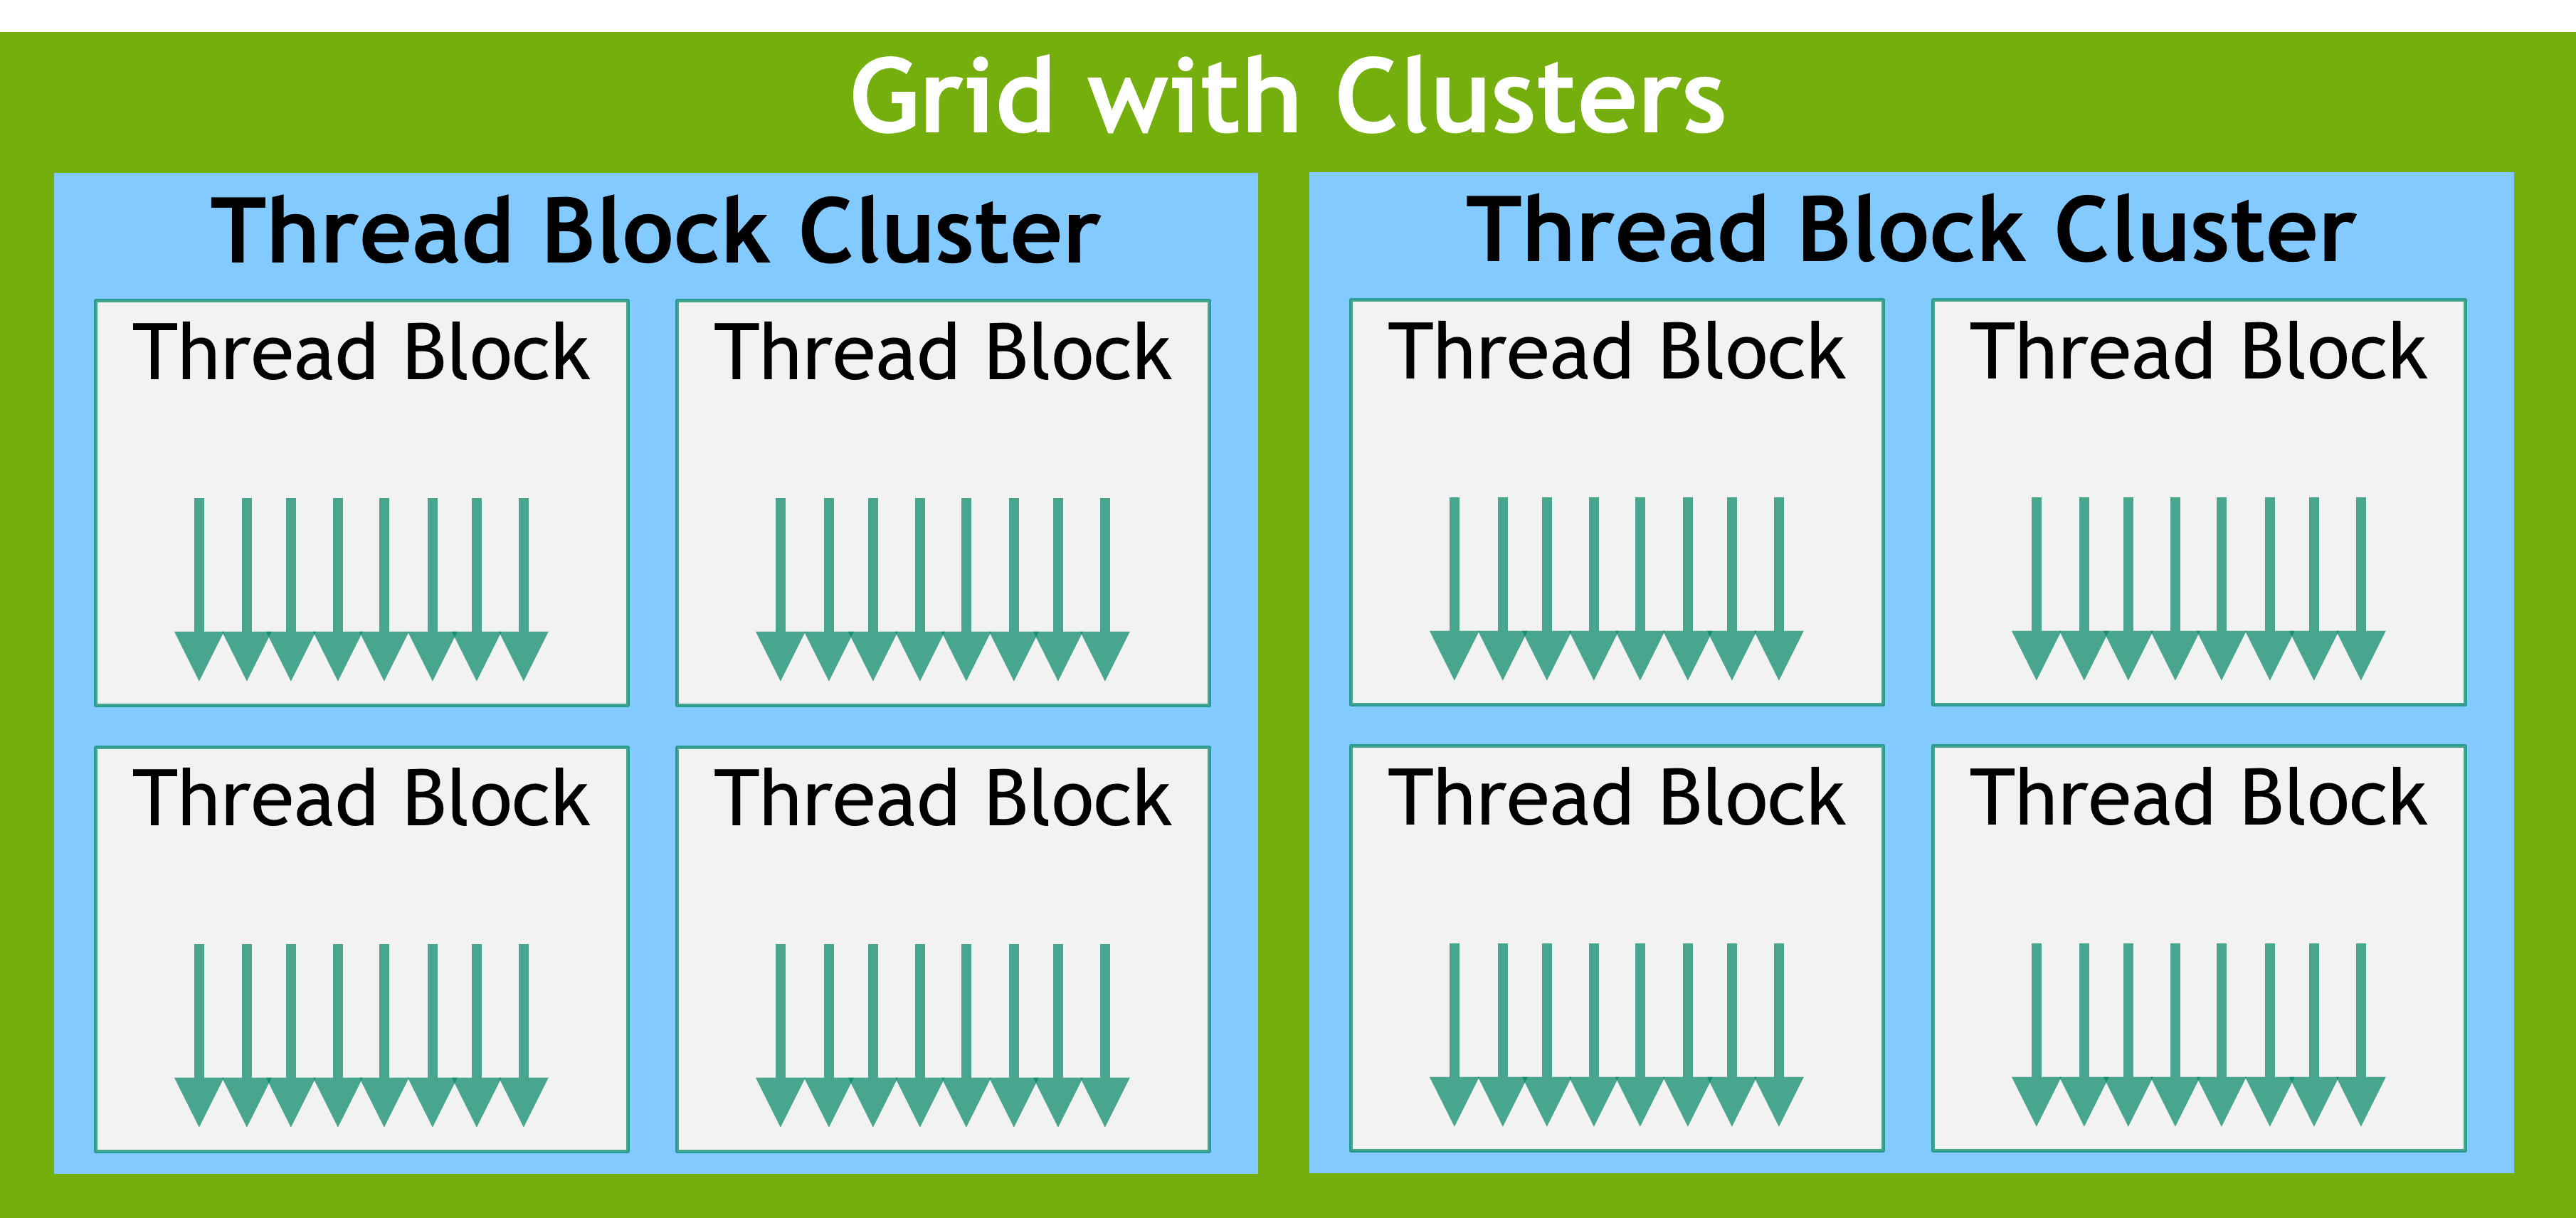
\includegraphics[width=0.7\linewidth]{Imagenes/Bitmap/grid}
	\caption{Cuadrícula de bloques de hilos}
	\label{fig:grid}
\end{figure}


Un bloque es un conjunto de hilos (que se distribuyen en tres dimensiones) que, como máximo, puede tener 1024 hilos diferentes por motivos de implementación en memoria (podemos tener un bloque de 1024x1x1 o 256x2x2 por ejemplo, pero no de 256x4x2, ya que el límite se refiere a la cantidad total de hilos, no al máximo en cada dimensión).

Podemos tener tantos bloques como queramos, organizados a su vez en la cuadrícula (también tridimensional). En cada hilo podemos acceder al índice de su bloque y del hilo dentro del bloque con \emph{blockIdx.dim} y \emph{threadIdx.dim} respectivamente, siendo dim la dimensión, osea x, y o z.

Aunque a nivel de usuario pueda parecer enrevesada esta distribución, esto está estrechamente relacionado con la implementación y la memoria compartida como podemos observar en la imagen \ref{fig:mem}. Todos los hilos tienen su propia memoria privada y una memoria compartida entre los demás hilos de su bloque, pero para compartir memoria con otros bloques hay que utilizar otros mecanismos que pueden afectar al rendimiento, luego implementar los hilos de manera adecuada puede hacer más eficientes los programas.

\begin{figure}
	\centering
	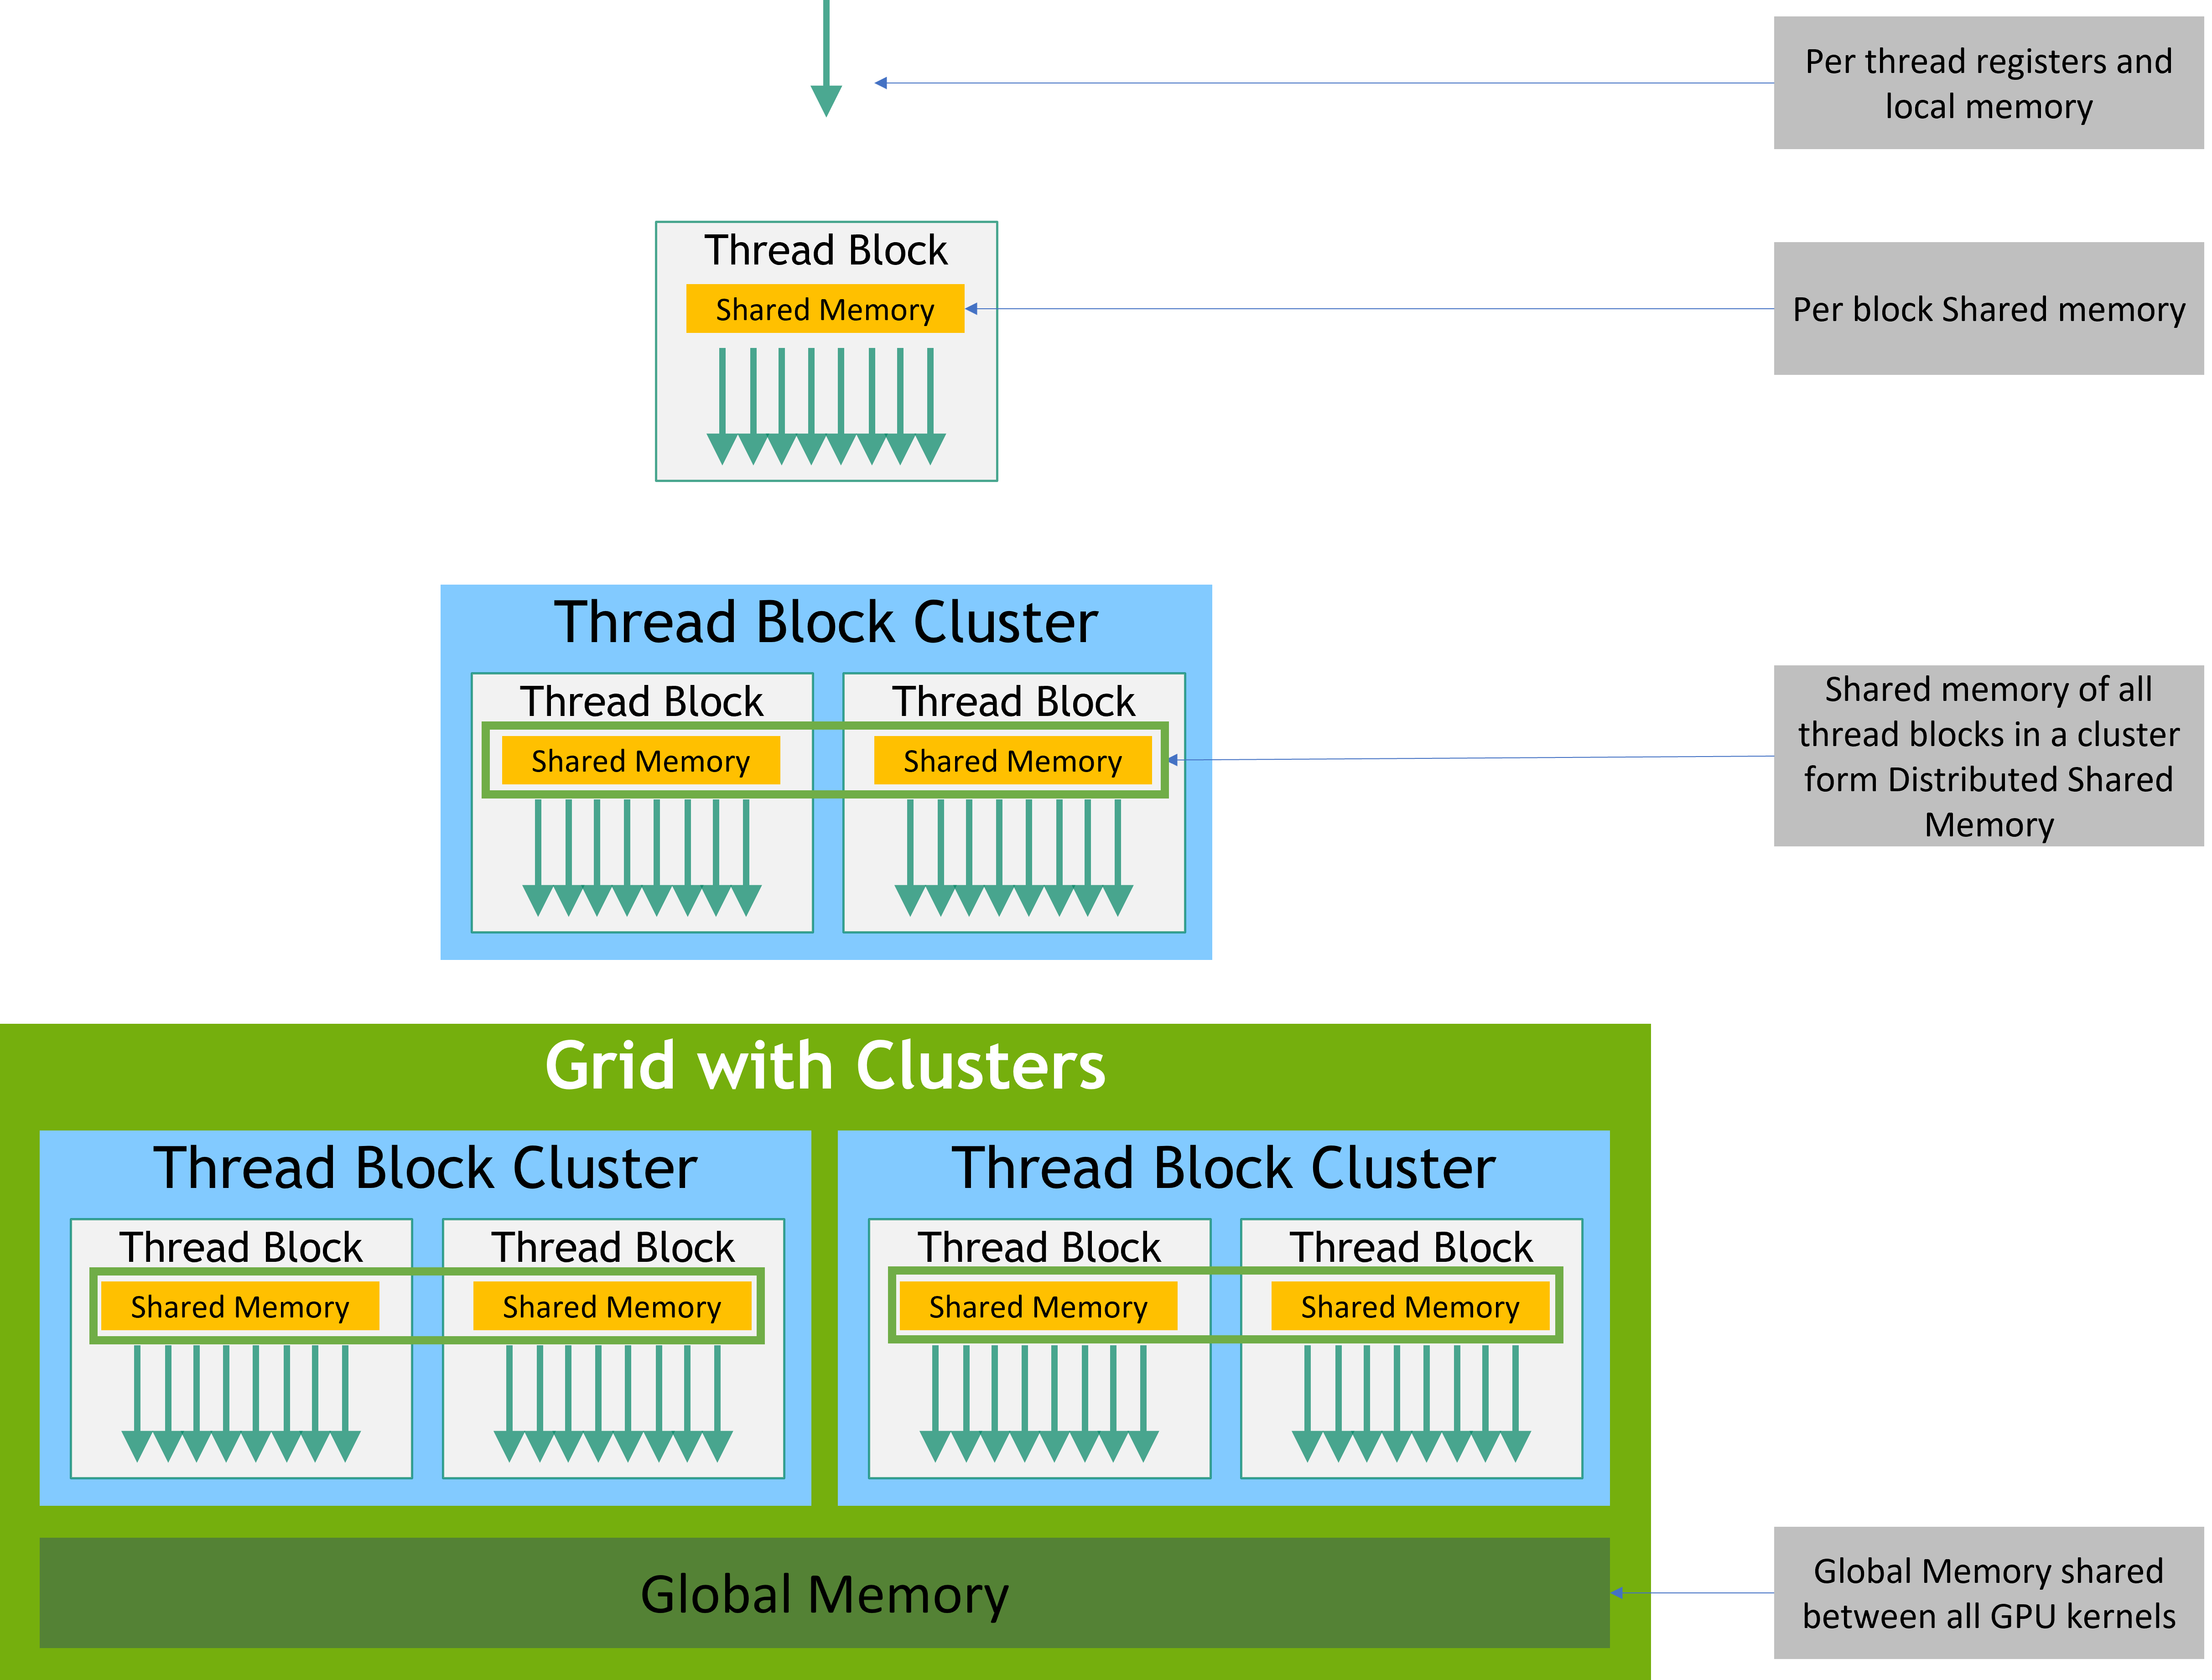
\includegraphics[width=0.7\linewidth]{Imagenes/Bitmap/memory}
	\caption{Memoria compartida entre elementos}
	\label{fig:mem}
\end{figure}


\section{Ejemplos}
Procedemos ahora a hacer un par de ejemplos sencillos que nos permitan familiarizarnos con estos conceptos.

\subsection{Hola Mundo}
Como es costumbre a la hora de programar, lo primero es hacer un "hola mundo", un programa que escriba en la consola la frase "hola mundo". Como el objetivo es poner de manifiesto que las cosas se están ejecutando varias veces en la \ac{GPU}, escribiremos el texto dos veces.

$\bullet$ En \ref{code:HelloWorldPY} vemos un ejemplo de uso de \textit{generateMod.py}, así como las funciones para reservar y copiar memoria en pycuda. Es importante destacar que a la hora de llamar al kernel desde la CPU, le tenemos que indicar qué forma va a tener cada uno de los bloques (osea, el número de hilos y cómo van a estar repartidos a lo largo de sus dimensiones).

$\bullet$ En \ref{code:HelloWorldCU} podemos ver la implementación del hola mundo en \ac{CUDA}, con el uso de la etiqueta \textbf{\_\_global\_\_} mencionada anteriormente.

$\bullet$ En \ref{code:HelloWorldOUT} vemos que la salida es la esperada.

\subsection{Suma de vectores}
Habiendo tenido ya nuestro primer contacto con pycuda, vamos ahora a poner de manifiesto la mejora de rendimiento que se puede conseguir. Vamos a realizar la suma de dos vectores de tamaños incrementalmente grandes, primero en CPU y luego en GPU, y vamos a comparar los tiempos que tarda en hacer ambas cosas.

$\bullet$ En \ref{code:vectorAddPY} podemos ver un ejemplo más complejo de código Python usando pycuda. La función \textit{add\_random\_vects} genera dos vectores de números aleatorios y los suma, primero en la CPU, y luego en GPU, midiendo el tiempo de ambos. Hay que destacar un par de cosas importantes:

Por un lado, hay que hacer la gestión de memoria, osea reservar memoria en GPU y copiar los datos con las funciones de pycuda. Por otro lado hay que gestionar el tamaño de bloque. Recordemos que los bloques pueden tener a lo sumo 1024 hilos, mientras que las grids pueden ser arbitrariamente grandes\footnote{En realidad hay un límite de tamaño dependiente del hardware, pero es tan grande que puede desestimarse}, esto implica que podríamos simplemente ejecutar un hilo por bloque y tantas mallas como el tamaño del vector, pero si recordamos la imagen \ref{fig:mem} podemos observar que los hilos de cada bloque comparten memoria local, por lo que si hacemos el máximo uso posible de los bloques (osea tratar con bloques de 1024 hilos), haremos un menor uso de la memoria y, por tanto, obtendremos resultados notablemente mejores.

Por último, comprobamos que las sumas coincidan y mostramos el incremento de eficiencia. Al ejecutar este script, simplemente llamamos a la función para valores de n entre $1$ y $10^{10}$

$\bullet$ En \ref{code:vectorAddCU} el código es bastante inmediato, calculamos el índice al que le corresponde nuestro hilo concreto y hacemos la suma. Solo hay una sutileza, y es que, en el último bloque que utilicemos, probablemente algunos hilos estén trabajando posiciones no válidas (porque todos los bloques tienen la misma cantidad de hilos, luego hay más hilos que posiciones en el vector). Para no acceder a posiciones de memoria posiblemente inválidas, simplemente añadimos a los datos de entrada el tamaño del vector y, si el hilo tiene un índice superior al tamaño del vector, no hacemos nada.

$\bullet$ En \ref{code:vectorAddOUT} se pone de manifiesto la mejora en la eficiencia, y es que cuando el tamaño del vector es suficientemente grande, el algoritmo es unas 10 veces más rápido. 





\chapter{Ecuación del calor}
\label{cap:heat}
\begin{resumen}
	En este capítulo desarrollaremos dos métodos numéricos, basados en las diferencias finitas, para aproximar la solución a la ecuación del calor en una  y dos dimensiones.
\end{resumen}

\section{Caso lineal}
En el caso unidimensional, tenemos la ecuación

\begin{equation}\label{eq:1dheat}
	\frac{\partial u}{\partial t} = \frac{\partial ^2u}{\partial x^2}
\end{equation}

Se pueden pedir diferentes condiciones iniciales para asegurar la existencia y unicidad de la ecuación \ref{eq:1dheat}, pero nosotros utilizaremos en concreto las condiciones
\begin{equation}
	\begin{cases}
			u(x,0)=f(x), \hspace{20px} a\leq x \leq b, \\
			u(a,t)=\alpha(t), \hspace{20px} 0<t, \\
			u(b,t)=\beta(t), \hspace{20px} 0<t.
	\end{cases}
\end{equation}

El problema de valor inicial que hemos definido tiene como dominio un rectángulo con uno de sus lados abierto hacia el infinito. Si fijamos $T>0$ tenemos ahora el rectángulo con el que trabajaremos. Definimos pues $B_T$ como la frontera del rectángulo y $D_T$ el interior de este, y por último definimos $D=D_T\cup B_T$.

\subsection{Existencia y unicidad}

Antes de estudiar la existencia y unicidad de la solución, necesitamos definir un concepto.
\begin{definicion}[Función continua a trozos]
	Una función es continua a trozos si es continua en todos sus puntos salvo en una cantidad finita.
\end{definicion}

Ahora enunciamos unas condiciones para la unicidad de las soluciones

\begin{teorema}[Unicidad]
	Sean $u$ y $v$ soluciones de la ecuación \ref{eq:1dheat} en $D_T$ continuas en $D$, si $u=v$ en $B_T$ entonces $u=v$ en $D$
\end{teorema}

\begin{teorema}[Unicidad extendida]
	Sean $u$ y $v$ soluciones de la ecuación \ref{eq:1dheat} en $D_T$ continuas a trozos en $D$ con una cantidad finita de discontinuidades acotadas, si $u=v$ en $B_T$ (excepto los puntos de discontinuidad) entonces $u=v$ en $D$
\end{teorema}

Estos teoremas nos dicen que basta con comprobar que todas las soluciones coinciden en la frontera del rectángulo para ver que la solución es única.

\begin{proof}
	Ver \citet{1dheat}, p.22
\end{proof}



\begin{teorema}[Existencia y unicidad]\label{teo:exis_uni_1dheat}
	Sean f, $\alpha$ y $\beta$ funciones continuas a trozos, la función
	
	\begin{multline}\label{eq:sol1dheat}
		u(x,t) = \int_{a}^{b}\theta(x-\xi,t)-\theta(x+\xi,t)f(\xi)d\xi \\
		- 2\int_{0}^{t}\frac{\partial \theta}{\partial x}(x, t-\tau)\alpha(\tau)d\tau+2\int_{0}^{t}\frac{\partial\theta}{\partial x}(x-1,t-\tau)\beta(\tau)d(\tau)
	\end{multline}
	
	donde $\theta(x,t)$ y $K(x,t)$ se definen como
	\[
		\theta(x,t)=\sum_{m=-\infty}^{\infty}K(x+2m,t) \hspace{15px} t>0
	\]\[
		K(x,t)=\frac{e^{\frac{-x^2}{4t}}}{\sqrt{4\pi t}}\hspace{15px} t>0
	\]
	
	Es la única solución acotada del problema del valor inicial
	\begin{equation}\label{eq:pvi1dheat}
		\begin{cases}
			\frac{\partial u}{\partial t} = \frac{\partial ^2u}{\partial x^2} \hspace{20px}a<x<b, \hspace{10px} 0<t, \\
			u(x,0)=f(x), \hspace{15px} a<x<b, \\
			u(a,t)=\alpha(t), \hspace{15px} 0<t, \\
			u(b,t)=\beta(t), \hspace{15px} 0<t.
		\end{cases}
	\end{equation}
	
\end{teorema}

\begin{proof}
	Puede verse en \cite{1dheat} que en efecto \ref{eq:sol1dheat} es solución de la ecuación del calor, por lo que solo tenemos que preocuparnos por la unicidad. Esto es inmediato por el teorema \ref{teo:exis_uni_1dheat}, ya que las condiciones iniciales fijan el valor de cualquier solución en $B_T$.
\end{proof}

Ahora podemos asegurar que \ref{eq:pvi1dheat} tiene una única solución, por lo que podemos proceder a aproximarla con un método de diferencias finitas.

\subsection[Aproximación de la solución]{Aproximación de la solución\footnote{Las demostraciones de toda esta sección son modificaciones propias de \cite{1dheat}, con el fin de hacerlas lo más sencillas posibles.}}
Utilizando la notación descrita en la sección \ref{sec:notacion}, aproximaremos la ecuación \ref{eq:1dheat} por el cociente incremental
\begin{multline} \label{eq:principio_aprox}
	u_t(x,t) = u_{x\bar{x}}(x,t) \Rightarrow \frac{u(x,t+\Delta t)-u(x,t)}{\Delta t} = \frac{1}{\Delta x^2}[u(x+\Delta x,t)-2u(x,t)+u(x-\Delta x, t)]
\end{multline}
Ahora, si nos ceñimos a una malla de puntos como definimos en \ref{sec:notacion}, siendo $\Delta t$ y $\Delta x$ el incremento entre los puntos de cada dimensión, tendremos:
\begin{equation}
	\frac{u_{i,j+1}-u_{i,j}}{\Delta t} = \frac{1}{\Delta x^2}[u_{i+1,j}-2u_{i,j}+u_{i-1,j}] \hspace{20px}\forall j\in \mathbb{N}^{+}
\end{equation}
Lo que, despejando y definiendo $\lambda \equiv \frac{\Delta t}{\Delta x^2}$ nos lleva a la fórmula explícita
\begin{equation}\label{eq:1dheat_formula}
	u_{i,j+1} = (1-2\lambda)u_{i,j}+\lambda(u_{i+1,j}+u_{i-1,j}) \hspace{20px} \forall j\in\mathbb{N}^+
\end{equation}

Analicemos un poco la fórmula \ref{eq:1dheat_formula}. Queremos calcular una aproximación de la solución en los puntos de la malla para $a\leq x\leq b$ y $0\leq t$.

Gracias al PVI tenemos los valores de $u_{i,0}$, $u_{0,j}$ y $u_{N,j} \hspace{5px}\forall i,j>=0$ (siendo $N$ tal que $b=a+N\Delta x$). Con esos valores está claro que podemos utilizar la fórmula \ref{eq:1dheat_formula} en todos los puntos de la malla.

\begin{figure}[h]
	\centering
	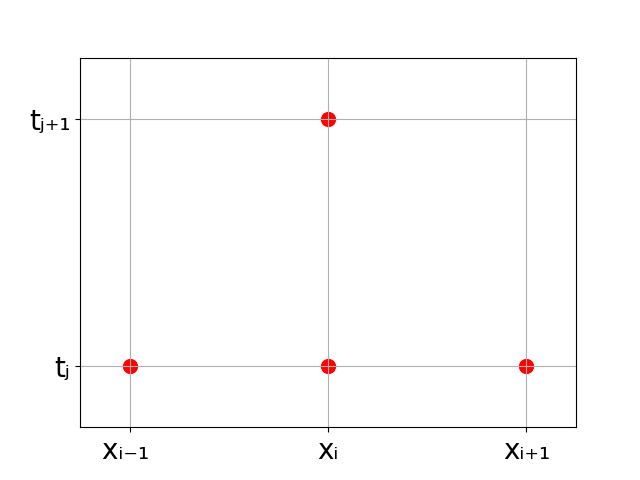
\includegraphics[scale=0.5]{./Imagenes/Bitmap/1dheat.png}
	\caption{Representación en la malla del esquema \ref{eq:1dheat_formula}}
\end{figure}

Para estudiar la convergencia de \ref{eq:1dheat_formula}, primero estudiaremos el siguiente lema:

\begin{lema}
	Suponiendo que $u$ es suficientemente diferenciable, se tiene que
	\begin{equation}
		\label{eq:lema1_eq1}
		u_t(x,t)-u_{x,\bar{x}}(x,t) = \tau(x,t)
	\end{equation}
	donde $t$ es el error de truncamiento, definido como
	\begin{equation}
		\label{eq:lema1_eq2}
		\tau(x,t) = \frac{\Delta t}{2}\frac{\partial^2 u}{\partial t^2} + \frac{\Delta x^2}{12}\frac{\partial^4u}{\partial x^4} + \xi_{\Delta x, \Delta t}.
	\end{equation}
	Siendo $\xi_{\Delta x, \Delta t}$ un número real que cumple que
	\begin{equation*}
		\xi_{\Delta x, \Delta t} \xrightarrow[\Delta x \rightarrow 0, \Delta t\rightarrow 0]{} 0 
	\end{equation*}
	
\end{lema}

\begin{proof}
	Haciendo el desarrollo de Taylor de orden 2 para la función $u$ con centro en el punto $(x,t)$ tenemos
	\begin{equation*}
		\begin{split}
		u(x,t+\Delta t)=u(x,t) + \frac{\partial u}{\partial t}\Delta t + \frac{1}{2}\frac{\partial^2u}{\partial t^2}\Delta t^2 + \xi^1_{\Delta x, \Delta t}\Delta t^2 \Rightarrow \\
		u_t(x,t) - \frac{\partial u}{\partial t} = \frac{\Delta t^2}{2}\frac{\partial^2u}{\partial t^2}\Delta t + \xi_{\Delta x, \Delta t}^1\Delta t
		\end{split}
	\end{equation*}
	Siendo $\xi^1$ un número con las mismas propiedades que $\xi$.
	Despejando la última ecuación, obtenemos el primer sumando de \ref{eq:lema1_eq1}, así como el de la ecuación \ref{eq:lema1_eq2}, y nos sobra $- \frac{\partial u}{\partial t}$ a la izquierda y $\xi_{\Delta x, \Delta t}^1\Delta t$ a la derecha.
	
	Si ahora hacemos los desarrollos de Taylor de orden 4 para la misma función pero en otros puntos, obtenemos
	\begin{equation*}
		u(x+\Delta x,t)=u(x,t)+\frac{\partial u}{\partial x}\Delta x+\frac{1}{2!}\frac{\partial^2 u}{\partial x^2}\Delta x^2 + \frac{1}{3!}\frac{\partial^3u}{\partial x^3}\Delta x^3+\frac{1}{4!}\frac{\partial^4u}{\partial x^4}\Delta x^4 + \xi_{\Delta x, \Delta t}^2\Delta x^4
	\end{equation*}
	y
	\begin{equation*}
		u(x-\Delta x,t)=u(x,t)-\frac{\partial u}{\partial x}\Delta x+\frac{1}{2!}\frac{\partial^2 u}{\partial x^2}\Delta x^2 - \frac{1}{3!}\frac{\partial^3u}{\partial x^3}\Delta x^3+\frac{1}{4!}\frac{\partial^4u}{\partial x^4}\Delta x^4 + \xi_{\Delta x, \Delta t}^3\Delta x^4
	\end{equation*}
	Siendo $\xi_{\Delta x, \Delta t}^2$ y $\xi_{\Delta x, \Delta t}^3$ números que cumplen las mismas propiedades que $\xi$.
	Ahora, si sumamos las dos últimas ecuaciones, ya que se nos cancelan los términos con exponente impar, obtenemos
	\begin{equation*}
		u_{x,\bar{x}} - \frac{\partial^2u}{\partial x^2}=\frac{1}{12}\frac{\partial^2u}{\partial x}\Delta x^2 + (\xi_{\Delta x, \Delta t}^2+\xi_{\Delta x, \Delta t}^3)\Delta x^2
	\end{equation*}

	Si restamos todo, tendiendo en cuenta que $\frac{\partial u}{\partial t} - \frac{\partial^2u}{\partial x^2}=0$, obtenemos precisamente la igualdad \ref{eq:lema1_eq1}, siendo $\xi_{\Delta x, \Delta t} = \xi_{\Delta x, \Delta t}^1\Delta t - (\xi_{\Delta x, \Delta t}^2+\xi_{\Delta x, \Delta t}^3)\Delta x^2$, por lo que se confirma que tiende a 0 cuando los incrementos tienden a 0.
\end{proof}

\begin{teorema}
	Si $0<\lambda<\frac{1}{2}$, el método numérico \ref{eq:1dheat_formula} es convergente, o dicho de otra forma, si $\epsilon_{i,j}$ es el error de aproximación del método, $\sup_{i,j}\epsilon(i,j)\rightarrow0$ si $\Delta t, \Delta x \rightarrow 0$ y el error inicial tiende a 0.
\end{teorema}



\begin{proof}
	Teniendo en cuenta el lema anterior, si ahora repetimos las cuentas de \ref{eq:principio_aprox} obtendríamos \ref{eq:1dheat_formula} pero añadiendo el sumando $\Delta t\tau_{i,j}$, por lo que cada vez que utilizamos esa fórmula estamos añadiendo ese error. Por ello, podemos deducir que
	\begin{equation*}
		\epsilon_{i,j+1} = (1-2\lambda)\epsilon_{i,j}+\lambda(\epsilon_{i+1,j}+\epsilon_{i-1,j})+ \Delta t\tau_{i,j}
	\end{equation*}
	Ahora, si definimos
	\begin{equation*}
		E_j=\sup_{i}|\epsilon_{i,j}|\hspace{30px}\tau=\sup_{i,j}|\tau_{i,j}|
	\end{equation*}
	tenemos que
	\begin{equation*}
		E_j+1\leq E_j+\Delta t\tau
	\end{equation*}
	por tanto, mediante una inducción trivial tenemos que
	\begin{equation*}
		E_j \leq E_0 + j\Delta t\tau = E_0+t_j\tau\hspace{15px}\forall j\geq0
	\end{equation*}
	
	Con esto ya tenemos el resultado, pues está claro, por su definición, que $\tau$ tiende a 0 cuando $\Delta t, \Delta x$ tienden a 0, luego el error está acotado por algo que tiende a 0, lo que implica que tiende a 0.
\end{proof}

\section{Caso bidimensional}

En el caso bidimensional, la ecuación que tenemos será
\begin{equation}\label{eq:2dheat}
	\frac{\partial u}{\partial t}=\frac{\partial^2u}{\partial x^2}+\frac{\partial^2u}{\partial y^2}
\end{equation}

\com{Voy a dejar esto en stand by, estoy teniendo problemas para encontrar algún teorema de existencia y unicidad para alguna condición inicial, y por tanto no sé que condiciones iniciales voy a acabar pidiéndole.}





%\include{Capitulos/Capitulo4}
%\include{Capitulos/Capitulo5}
%\chapter{Conclusiones y Trabajo Futuro}
\label{cap:conclusiones}

Conclusiones del trabajo y líneas de trabajo futuro.

Antes de la entrega de actas de cada convocatoria, en el plazo que se indica en el calendario de los trabajos de fin de grado, el estudiante entregará en el Campus Virtual la versión final de la memoria en PDF.




%%%%%%%%%%%%%%%%%%%%%%%%%%%%%%%%%%%%%%%%%%%%%%%%%%%%%%%%%%%%%%%%%%%%%%%%%%%
% Si el TFG se escribe en inglés, comentar las siguientes líneas 
% porque no es necesario incluir nuevamente las Conclusiones en inglés
\begin{otherlanguage}{english}
%\chapter*{Introduction}
\label{cap:introduction}
\addcontentsline{toc}{chapter}{Introduction}

Introduction to the subject area. This chapter contains the translation of Chapter \ref{cap:introduccion}.










%\chapter*{Conclusions and Future Work}
\label{cap:conclusions}
\addcontentsline{toc}{chapter}{Conclusions and Future Work}

Conclusions and future lines of work. This chapter contains the translation of Chapter \ref{cap:conclusiones}.



\end{otherlanguage}
%%%%%%%%%%%%%%%%%%%%%%%%%%%%%%%%%%%%%%%%%%%%%%%%%%%%%%%%%%%%%%%%%%%%%%%%%%%

%\include{Capitulos/ContribucionesPersonales}

%
% Bibliografía
%
% Si el TFM se escribe en inglés, editar TeXiS/TeXiS_bib para cambiar el
% estilo de las referencias
%---------------------------------------------------------------------
%
%                      configBibliografia.tex
%
%---------------------------------------------------------------------
%
% bibliografia.tex
% Copyright 2009 Marco Antonio Gomez-Martin, Pedro Pablo Gomez-Martin
%
% This file belongs to the TeXiS manual, a LaTeX template for writting
% Thesis and other documents. The complete last TeXiS package can
% be obtained from http://gaia.fdi.ucm.es/projects/texis/
%
% Although the TeXiS template itself is distributed under the 
% conditions of the LaTeX Project Public License
% (http://www.latex-project.org/lppl.txt), the manual content
% uses the CC-BY-SA license that stays that you are free:
%
%    - to share & to copy, distribute and transmit the work
%    - to remix and to adapt the work
%
% under the following conditions:
%
%    - Attribution: you must attribute the work in the manner
%      specified by the author or licensor (but not in any way that
%      suggests that they endorse you or your use of the work).
%    - Share Alike: if you alter, transform, or build upon this
%      work, you may distribute the resulting work only under the
%      same, similar or a compatible license.
%
% The complete license is available in
% http://creativecommons.org/licenses/by-sa/3.0/legalcode
%
%---------------------------------------------------------------------
%
% Fichero  que  configura  los  parámetros  de  la  generación  de  la
% bibliografía.  Existen dos  parámetros configurables:  los ficheros
% .bib que se utilizan y la frase célebre que aparece justo antes de la
% primera referencia.
%
%---------------------------------------------------------------------


%%%%%%%%%%%%%%%%%%%%%%%%%%%%%%%%%%%%%%%%%%%%%%%%%%%%%%%%%%%%%%%%%%%%%%
% Definición de los ficheros .bib utilizados:
% \setBibFiles{<lista ficheros sin extension, separados por comas>}
% Nota:
% Es IMPORTANTE que los ficheros estén en la misma línea que
% el comando \setBibFiles. Si se desea utilizar varias líneas,
% terminarlas con una apertura de comentario.
%%%%%%%%%%%%%%%%%%%%%%%%%%%%%%%%%%%%%%%%%%%%%%%%%%%%%%%%%%%%%%%%%%%%%%
\setBibFiles{%
libros, otros%
}

%%%%%%%%%%%%%%%%%%%%%%%%%%%%%%%%%%%%%%%%%%%%%%%%%%%%%%%%%%%%%%%%%%%%%%
% Definición de la frase célebre para el capítulo de la
% bibliografía. Dentro normalmente se querrá hacer uso del entorno
% \begin{FraseCelebre}, que contendrá a su vez otros dos entornos,
% un \begin{Frase} y un \begin{Fuente}.
%
% Nota:
% Si no se quiere cita, se puede eliminar su definición (en la
% macro setCitaBibliografia{} ).
%%%%%%%%%%%%%%%%%%%%%%%%%%%%%%%%%%%%%%%%%%%%%%%%%%%%%%%%%%%%%%%%%%%%%%
\setCitaBibliografia{
\begin{FraseCelebre}
\begin{Frase}
  Y así, del mucho leer y del poco dormir, se le secó el celebro de
  manera que vino a perder el juicio.
\end{Frase}
\begin{Fuente}
  Miguel de Cervantes Saavedra
\end{Fuente}
\end{FraseCelebre}
}

%%
%% Creamos la bibliografia
%%
\makeBib

% Variable local para emacs, para  que encuentre el fichero maestro de
% compilación y funcionen mejor algunas teclas rápidas de AucTeX

%%%
%%% Local Variables:
%%% mode: latex
%%% TeX-master: "../Tesis.tex"
%%% End:



% Apéndices
\appendix


\chapter{Código}
\label{Appendix:codigo}
\lstinputlisting[label=code:generateMod, caption=Módulo para generar SourceModule a partir de los archivos]{../Codigo/python/generateMod.py}
 
%HelloWorld

\lstinputlisting[label=code:HelloWorldPY, caption=Hola Mundo (Código Python)]{../Codigo/python/HelloWorld.py}
\lstinputlisting[label=code:HelloWorldCU, caption=Hola Mundo (Código CUDA), language=C++]{../Codigo/CUDA/HelloWorld.cu}
\lstinputlisting[label=code:HelloWorldOUT, caption=Hola Mundo (Salida), language=]{../Codigo/out/HelloWorld.out}

%vectorAdd

\lstinputlisting[label=code:vectorAddPY, caption=Suma de vectores (Código Python), lastline=42]{../Codigo/python/vectorAdd.py}
\lstinputlisting[label=code:vectorAddCU, caption=Suma de vectores (Código CUDA), language=C++]{../Codigo/CUDA/vectorAdd.cu}
\lstinputlisting[label=code:vectorAddOUT, caption=Suma de vectores (Salida), language=]{../Codigo/out/vectorAdd.out}

%heat1D
\lstinputlisting[label=code:heat1D_py, caption=Método numérico para la ecuación del calor en 1D (Código Python)]{../Codigo/python/heat1d.py}
\lstinputlisting[label=code:heat1DGPU_py, caption=Método numérico para la ecuación del calor en 1D utilizando CUDA (Código Python)]{../Codigo/python/heat1Dgpu.py}
\lstinputlisting[label=code:heat1DGPU_cu, caption=Kernel para calcular el resultado de una fila concreta (supuesto que las anteriores estén ya hechas),language=C++]{../Codigo/CUDA/heat1d.cu}


%wave 1D
\lstinputlisting[label=code:wave1D_py, caption=Método numérico para la ecuación de onda en 1D (Código Python)]{../Codigo/python/wave1d.py}
%\chapter{Título del Apéndice B}
\label{Appendix:Key2}

Se pueden añadir los apéndices que se consideren oportunos.
%\include{Apendices/appendixC}
%\include{...}
%\include{...}
%\include{...}
\backmatter



%
% Índice de palabras
%

% Sólo  la   generamos  si  está   declarada  \generaindice.  Consulta
% TeXiS.sty para más información.

% En realidad, el soporte para la generación de índices de palabras
% en TeXiS no está documentada en el manual, porque no ha sido usada
% "en producción". Por tanto, el fichero que genera el índice
% *no* se incluye aquí (está comentado). Consulta la documentación
% en TeXiS_pream.tex para más información.
\ifx\generaindice\undefined
\else
%%---------------------------------------------------------------------
%
%                        TeXiS_indice.tex
%
%---------------------------------------------------------------------
%
% TeXiS_indice.tex
% Copyright 2009 Marco Antonio Gomez-Martin, Pedro Pablo Gomez-Martin
%
% This file belongs to TeXiS, a LaTeX template for writting
% Thesis and other documents. The complete last TeXiS package can
% be obtained from http://gaia.fdi.ucm.es/projects/texis/
%
% This work may be distributed and/or modified under the
% conditions of the LaTeX Project Public License, either version 1.3
% of this license or (at your option) any later version.
% The latest version of this license is in
%   http://www.latex-project.org/lppl.txt
% and version 1.3 or later is part of all distributions of LaTeX
% version 2005/12/01 or later.
%
% This work has the LPPL maintenance status `maintained'.
% 
% The Current Maintainers of this work are Marco Antonio Gomez-Martin
% and Pedro Pablo Gomez-Martin
%
%---------------------------------------------------------------------
%
% Contiene  los  comandos  para  generar  el índice  de  palabras  del
% documento.
%
%---------------------------------------------------------------------
%
% NOTA IMPORTANTE: el  soporte en TeXiS para el  índice de palabras es
% embrionario, y  de hecho  ni siquiera se  describe en el  manual. Se
% proporciona  una infraestructura  básica (sin  terminar)  para ello,
% pero  no ha  sido usada  "en producción".  De hecho,  a pesar  de la
% existencia de  este fichero, *no* se incluye  en Tesis.tex. Consulta
% la documentación en TeXiS_pream.tex para más información.
%
%---------------------------------------------------------------------


% Si se  va a generar  la tabla de  contenidos (el índice  habitual) y
% también vamos a  generar el índice de palabras  (ambas decisiones se
% toman en  función de  la definición  o no de  un par  de constantes,
% puedes consultar modo.tex para más información), entonces metemos en
% la tabla de contenidos una  entrada para marcar la página donde está
% el índice de palabras.

\ifx\generatoc\undefined
\else
   \addcontentsline{toc}{chapter}{\indexname}
\fi


% Generamos el índice
\printindex

% Variable local para emacs, para  que encuentre el fichero maestro de
% compilación y funcionen mejor algunas teclas rápidas de AucTeX

%%%
%%% Local Variables:
%%% mode: latex
%%% TeX-master: "./tesis.tex"
%%% End:

\fi

%
% Lista de acrónimos
%

% Sólo  lo  generamos  si  está declarada  \generaacronimos.  Consulta
% TeXiS.sty para más información.


\ifx\generaacronimos\undefined
\else
%---------------------------------------------------------------------
%
%                        TeXiS_acron.tex
%
%---------------------------------------------------------------------
%
% TeXiS_acron.tex
% Copyright 2009 Marco Antonio Gomez-Martin, Pedro Pablo Gomez-Martin
%
% This file belongs to TeXiS, a LaTeX template for writting
% Thesis and other documents. The complete last TeXiS package can
% be obtained from http://gaia.fdi.ucm.es/projects/texis/
%
% This work may be distributed and/or modified under the
% conditions of the LaTeX Project Public License, either version 1.3
% of this license or (at your option) any later version.
% The latest version of this license is in
%   http://www.latex-project.org/lppl.txt
% and version 1.3 or later is part of all distributions of LaTeX
% version 2005/12/01 or later.
%
% This work has the LPPL maintenance status `maintained'.
% 
% The Current Maintainers of this work are Marco Antonio Gomez-Martin
% and Pedro Pablo Gomez-Martin
%
%---------------------------------------------------------------------
%
% Contiene  los  comandos  para  generar  el listado de acrónimos
% documento.
%
%---------------------------------------------------------------------
%
% NOTA IMPORTANTE:  para que la  generación de acrónimos  funcione, al
% menos  debe  existir  un  acrónimo   en  el  documento.  Si  no,  la
% compilación  del   fichero  LaTeX  falla  con   un  error  "extraño"
% (indicando  que  quizá  falte  un \item).   Consulta  el  comentario
% referente al paquete glosstex en TeXiS_pream.tex.
%
%---------------------------------------------------------------------


% Redefinimos a español  el título de la lista  de acrónimos (Babel no
% lo hace por nosotros esta vez)

\def\listacronymname{Lista de acrónimos}

% Para el glosario:
% \def\glosarryname{Glosario}

% Si se  va a generar  la tabla de  contenidos (el índice  habitual) y
% también vamos a  generar la lista de acrónimos  (ambas decisiones se
% toman en  función de  la definición  o no de  un par  de constantes,
% puedes consultar config.tex  para más información), entonces metemos
% en la  tabla de contenidos una  entrada para marcar  la página donde
% está el índice de palabras.

\ifx\generatoc\undefined
\else
   \addcontentsline{toc}{chapter}{\listacronymname}
\fi


% Generamos la lista de acrónimos (en realidad el índice asociado a la
% lista "acr" de GlossTeX)

\printglosstex(acr)

% Variable local para emacs, para  que encuentre el fichero maestro de
% compilación y funcionen mejor algunas teclas rápidas de AucTeX

%%%
%%% Local Variables:
%%% mode: latex
%%% TeX-master: "../Tesis.tex"
%%% End:

\fi

%
% Final
%
%---------------------------------------------------------------------
%
%                      fin.tex
%
%---------------------------------------------------------------------
%
% fin.tex
% Copyright 2009 Marco Antonio Gomez-Martin, Pedro Pablo Gomez-Martin
%
% This file belongs to the TeXiS manual, a LaTeX template for writting
% Thesis and other documents. The complete last TeXiS package can
% be obtained from http://gaia.fdi.ucm.es/projects/texis/
%
% Although the TeXiS template itself is distributed under the 
% conditions of the LaTeX Project Public License
% (http://www.latex-project.org/lppl.txt), the manual content
% uses the CC-BY-SA license that stays that you are free:
%
%    - to share & to copy, distribute and transmit the work
%    - to remix and to adapt the work
%
% under the following conditions:
%
%    - Attribution: you must attribute the work in the manner
%      specified by the author or licensor (but not in any way that
%      suggests that they endorse you or your use of the work).
%    - Share Alike: if you alter, transform, or build upon this
%      work, you may distribute the resulting work only under the
%      same, similar or a compatible license.
%
% The complete license is available in
% http://creativecommons.org/licenses/by-sa/3.0/legalcode
%
%---------------------------------------------------------------------
%
% Contiene la última página
%
%---------------------------------------------------------------------


% Ponemos el marcador en el PDF
\ifpdf
   \pdfbookmark{Fin}{fin}
\fi

\thispagestyle{empty}\mbox{}

Este texto se puede encontrar en el fichero Cascaras/fin.tex. Si deseas eliminarlo, basta con comentar la línea correspondiente al final del fichero TFGTeXiS.tex.

\vspace*{4cm}

\small

\hfill \emph{--¿Qué te parece desto, Sancho? -- Dijo Don Quijote --}

\hfill \emph{Bien podrán los encantadores quitarme la ventura,}

\hfill \emph{pero el esfuerzo y el ánimo, será imposible.}

\hfill 

\hfill \emph{Segunda parte del Ingenioso Caballero} 

\hfill \emph{Don Quijote de la Mancha}

\hfill \emph{Miguel de Cervantes}

\vfill%space*{4cm}

\hfill \emph{--Buena está -- dijo Sancho --; fírmela vuestra merced.}

\hfill \emph{--No es menester firmarla -- dijo Don Quijote--,}

\hfill \emph{sino solamente poner mi rúbrica.}

\hfill 

\hfill \emph{Primera parte del Ingenioso Caballero} 

\hfill \emph{Don Quijote de la Mancha}

\hfill \emph{Miguel de Cervantes}


\newpage
\thispagestyle{empty}\mbox{}

\newpage

% Variable local para emacs, para  que encuentre el fichero maestro de
% compilación y funcionen mejor algunas teclas rápidas de AucTeX

%%%
%%% Local Variables:
%%% mode: latex
%%% TeX-master: "../Tesis.tex"
%%% End:

%\end{otherlanguage}
\end{document}
